% ------------------------------------------------------------------------ %
% Modello di tesi di laurea o di dottorato
% di Luca Maggiori ©
%
% basato sul modello proposto da Lorenzo Pantieri
% (http://www.lorenzopantieri.net/LaTeX.html)
% e con la possibilità di attivare le impostazioni
% di impaginazione previste dal Politecnico di Milano
%
% versione 1.0	-- 4 maggio 2014
%	- prima versione completa
% versione 1.1	-- 5 maggio 2014
%	- aggiunta codici di esempio
%	- attivazione elenco dei codici
% ------------------------------------------------------------------------ %
%
%
% ------------------------------------------------------------------------ %
% Le impostazioni specifiche per il Politecnico di Milano
% sono definite sulla base del seguente documento:
% http://www.ingind.polimi.it/cms/file/1262/Norme_per_la_stesura_di_tesi_di_laurea_specialistica.pdf
% già presente nella cartella AltroMateriale
%
% Alcune delle impostazioni sono commentate e sostituite
% da altre ritenute in qualche modo 'migliori'; possono
% essere ripristinate commentando/decommentando i vari comandi
% ------------------------------------------------------------------------ %
%
%
% ------------------------------------------------------------------------ %
% I seguenti commenti speciali impostano:
% - applemac come codifica di input,
% - PDFLaTeX come motore di composizione;
% - Tesi.tex come documento principale;
% - il controllo ortografico italiano per l'editor.
%
% !TEX encoding = UTF-8 Unicode
% !TEX TS-program = pdflatex
% !TEX root = Tesi.tex
% !TEX spellcheck = it-IT
% ------------------------------------------------------------------------ %
%
%
% ------------------------------------------------------------------------ %
% 	PREAMBOLO
% ------------------------------------------------------------------------ %
%
\documentclass[12pt,	% 10-11-12pt (12pt preferibile)
	a4paper,		%
	twoside,		% fronte-retro
	openright,		% nuovi capitoli iniziano nella pagina dispari
	titlepage,% 	% nuova pagina dopo il titolo (necessario per frontespizio)
	]{book}
%
% ------------------------------------------------------------------------ %
%
\usepackage[T1]{fontenc}		% codifica di output
%				% N.B. richiede una distribuzione completa di LaTeX
%
\usepackage{lmodern}
%
\usepackage[utf8]{inputenc}		% codifica di input; anche [latin1] va bene
%				% N.B. va accordata con le preferenze dell'editor
%
\usepackage[english,italian]{babel}	% scelta lingua, sillabazione...
%				% l'ultima lingua (italiano) sarà la predefinita
%
\usepackage{microtype}		% micro-tipografia
%
% ------------------------------------------------------------------------ %
%
% 	LAYOUT - MARGINI - RILEGATURA
%
% -- AUTOMATICO
\usepackage[binding=5mm]{layaureo} 	% margini ottimizzati per l'A4; rilegatura di 5 mm
%
% -- MANUALE (Impostazioni PoliMi)
%\usepackage{geometry}
%
%\geometry{verbose,	% verbose = displays the parameter results on the terminal
%	top=43mm,	% margine superiore (PoliMi=43mm)
%	bottom=44mm,	% margine inferiore (PoliMi=44mm)
%	inner=41mm,	% margine interno pagina (PoliMi=41mm)
%	outer=32mm,	% margine esterno pagina (PoliMi=32mm)
%	bindingoffset=5mm,	% margine per la rilegatura
%	heightrounded}
%
% ------------------------------------------------------------------------ %
%
\usepackage[swapnames]{frontespizio}	% frontespizio (elegante ma non previsto al PoliMi)
%		% per includerlo nel documento bisogna:
%		% 1. compilare una prima volta Tesi.tex;
%		% 2. compilare a parte Tesi-frn.tex, generato dalla compilazione precedente;
%		% 3. compilare ancora Tesi.tex.
%		% Non è necessario fare questi passaggi altre volte
%		% se il frontespizio non è più modificato.
%
\usepackage{changepage,calc}                 % centra il frontespizio
%
\usepackage{emptypage}		% pagine vuote senza testatina e piede di pagina
%
\usepackage{indentfirst}		% rientra il primo paragrafo di ogni sezione
%
\usepackage{booktabs}		% tabelle (\toprule, \midrule, \bottomrule)
%
\usepackage{tabularx}		% tabelle di larghezza prefissata
%
\usepackage{graphicx}		% immagini
%
\usepackage[figuresright]{rotating}	% tabelle a 90 gradi
%
\usepackage{subfig}			% sottofigure, sottotabelle
%
\usepackage{caption}		% didascalie
%
\usepackage{listings}		% codici
%
\usepackage[font=small]{quoting}	% citazioni
%
\usepackage{amsmath,amssymb}	% matematica
%
\usepackage{mathtools}		% matematica
%
\usepackage{amsthm}		% matematica
%
\usepackage[output-decimal-marker={,}]{siunitx}	% SI (con separatore decimale=virgola)
%
\usepackage[italian]{varioref}		% riferimenti completi, con indicazione della pagina (\vref)
%
\usepackage{mparhack,fixltx2e}	% finezze tipografiche (bug fixes di LaTeX)
%
\usepackage{relsize}			% make text larger or smaller than the surrounding text
% 				% \larger[i] \smaller[i]
%
% ------------------------------------------------------------------------ %
%
% 	BIBLIOGRAFIA
%
% ------------------------------------------------------------------------ %
%
% Per generare effettivamente la bibliografia nel documento
% questa è la sequenza di composizione:
% 1. si compone il documento con LATEX una prima volta;
% 2. si lancia il programma Biber premendo l’apposito pulsante dell’editor;
% 3. si compone il documento altre 2 volte con LATEX (ma anche 3, NdA)
% Tale sequenza deve essere ripetuta solo se vengono fatte modifiche/aggiunte
% al database bibliografico.
%
% ------------------------------------------------------------------------ %
%
\usepackage[dvipsnames]{xcolor}	% colori - 68 colori predefiniti:
% 				% http://en.wikibooks.org/wiki/LaTeX/Colors
%
\usepackage{lipsum}			% testo fittizio
%
\usepackage{eurosym}		% simbolo dell'euro
%
\usepackage{hyperref}		% collegamenti ipertestuali
%
\usepackage{bookmark}		% gestione segnalibri del PDF
%
\usepackage{guit}			% simboli del Guit
%
\usepackage{fancyhdr}		% testatine e piede personalizzati
\setlength{\headheight}{15pt}
%
\usepackage{colortbl}		% per colorare i filetti delle tabelle
%
\usepackage[footnote,		% descrizione acronimo fatta a piè di pagina
	smaller,			% acronimo scritto con dimensione ridotta
	]{acronym}		% acronimi
%
\usepackage{multirow}		% celle tabelle alte più di una riga
%
\usepackage{pdfpages}		% inclusione di files pdf esterni
%
% ------------------------------------------------------------------------ %
% 	MY PACKAGES
% ------------------------------------------------------------------------ %
%
\usepackage{float}
%
% ------------------------------------------------------------------------ %
% 	PREAMBOLO - SETUP
% ------------------------------------------------------------------------ %
%
% ------------------------------------------------------------------------ %
% !TEX encoding = UTF-8 Unicode
% !TEX TS-program = pdflatex
% !TEX root = Tesi.tex
% !TEX spellcheck = it-IT
% ------------------------------------------------------------------------ %
%
% ------------------------------------------------------------------------ %
% 	PREAMBOLO - SETUP
% ------------------------------------------------------------------------ %
% Comandi personali
% ------------------------------------------------------------------------ %
%
\newcommand{\myName}{Luca Maggiori}			% autore
\newcommand{\myMatricola}{783186}			% matricola
\newcommand{\myTitle}{Modello di Tesi di Laurea in \LaTeX{}}	% titolo
\newcommand{\myUni}{Politecnico di Milano}		% università
\newcommand{\myFaculty}{Scuola di Ingegneria Industriale e dell'Informazione}	% facoltà/scuola
\newcommand{\myDegree}{Ingegneria Meccanica}		% laurea
\newcommand{\myThesis}{Tesi di Laurea Magistrale}	% tipo di tesi
\newcommand{\myDepartment}{Dipartimento di Meccanica}	% dipartimento
\newcommand{\myProf}{Prof.~Charles~Dickens}		% relatore
\newcommand{\myOtherProf}{Ing.~Emilio~Salgari}		% eventuale correlatore
\newcommand{\myLocation}{Milano}			% dove
\newcommand{\myTime}{Aprile 2014}			% quando
\newcommand{\myAcademicYear}{2012--2013}		% anno accademico
\newcommand{\myLogo}{logoPoliMi}			% logo
\newcommand{\myLogoCFD}{logoPoliMiCFD}		% logo CFD :-)
\newcommand{\myUrlUni}{www.polimi.it}			% sito PoliMi
\newcommand{\myUrlFaculty}{www.ingindinf.polimi.it}	% sito Facoltà
%
% ------------------------------------------------------------------------ %
% Impostazioni di amsmath, amssymb, amsthm
% ------------------------------------------------------------------------ %
%
% un ambiente per i sistemi
\newenvironment{sistema}%
	{\left\lbrace\begin{array}{@{}l@{}}}%
	{\end{array}\right.}
%
% epsilon theta rho phi
\renewcommand{\epsilon}{\varepsilon}
\renewcommand{\theta}{\vartheta}
%\renewcommand{\rho}{\varrho}
\renewcommand{\phi}{\varphi}
%
\renewcommand{\vec}{\mathbf} 	% vettori in tondo nero
%
% ------------------------------------------------------------------------ %
% Impostazioni di biblatex
% ------------------------------------------------------------------------ %
%
% -- commentare o cancellare tutto se si desidera bibliografia standard
%
% I comandi seguenti saranno poi usati in Bibliografia.tex
% per suddividere i riferimenti bibliografici tra materiale citato
% e materiale non citato nel testo, con l'ulteriore distinzione in
% materiale cartaceo e materiale online (con link)
%
% Al termine si riportano anche pubblicazioni legate a Latex
% e alla stesura della tesi di laurea
%
\newcommand{\bibtitolocitati}{Riferimenti citati nel testo}
\newcommand{\bibtitolocitaticarta}{Pubblicazioni e Manuali}
\newcommand{\bibtitolocitatiweb}{Materiale Online}
\newcommand{\bibtitolononcitati}{Ulteriore materiale consultato}
\newcommand{\bibtitolononcitaticarta}{Pubblicazioni e Manuali}
\newcommand{\bibtitolononcitatiweb}{Materiale Online}
\newcommand{\bibtitololatex}{{\LaTeX{}}}
%
\DeclareBibliographyCategory{citati}
%
\defbibheading{citati-cartacei}{\subsection*{\bibtitolocitaticarta}}
\defbibheading{citati-web}{\subsection*{\bibtitolocitatiweb}}
\defbibheading{non-citati}{\section*{\bibtitolononcitati}}
\defbibheading{non-citati-cartacei}{\subsection*{\bibtitolononcitaticarta}}
\defbibheading{non-citati-web}{\subsection*{\bibtitolononcitatiweb}}
\defbibheading{latex}{\subsection*{\bibtitololatex}}
%
\AtEveryCitekey{\addtocategory{citati}{\thefield{entrykey}}}
%
\AtEveryBibitem{
    \clearfield{doi}
    \clearfield{eprint}
}
%
\nocite{*}	% manda in bibliografia anche tutte le opere non citate
%
% ------------------------------------------------------------------------ %
%
% Decommentare i comandi che seguono
% se si vuole ripristinare bibliografia standard
% (commentando tutto il blocco precedente)
%
%\defbibheading{bibliography}{%
%	\cleardoublepage%
%	\phantomsection%
%	\addcontentsline{toc}{chapter}{\bibname}%
%	\chapter*{\bibname\markboth{\bibname}{\bibname}}%
%	}
%
% ------------------------------------------------------------------------ %
% Impostazioni di xcolor
% ------------------------------------------------------------------------ %
%
% webcolors
\definecolor{webgreen}{rgb}{0,.5,0}
\definecolor{webbrown}{rgb}{.6,0,0}
%
% BluePolimi (colori delle presentazioni PPT del Politecnico di Milano)
\definecolor{darkbluePoliMi}{rgb}{0,0.18,0.40}	%rgb(0, 46, 103)
\definecolor{midbluePoliMi}{rgb}{0.33,0.47,0.62}	%rgb(84, 121, 157)
\definecolor{lightbluePoliMi}{rgb}{0.53,0.64,0.73}	%rgb(134, 163, 186)
\definecolor{orangePoliMi}{rgb}{1,0.59,0}		%rgb(255, 151, 0)
%
% redSapienza (rosso Sapienza)
\definecolor{redSapienza}{rgb}{0.514,0.031,0.165}	%rgb(131, 8, 42)
%
% ------------------------------------------------------------------------ %
% Impostazioni di listings
% ------------------------------------------------------------------------ %
%
\lstset{
	basicstyle=\smaller[0]\ttfamily,		% Black & White:
	keywordstyle=\color{RoyalBlue},	% keywordstyle=\color{black}\bfseries,
	commentstyle=\color{webgreen},	% commentstyle=\color{gray},
	stringstyle=\color{webbrown},		% stringstyle=\color{black},
	numbers=left,
	numberstyle=\smaller[2],
	stepnumber=1,
	numbersep=8pt,
	showspaces=false,
	showstringspaces=false,
	showtabs=false,
	breaklines=true,
	frameround=ffff,
	frame=single,
	tabsize=2,
	captionpos=t,
	breakatwhitespace=false,
	}
%
% Solution to the encoding issue
\lstset{literate=
  {á}{{\'a}}1 {é}{{\'e}}1 {í}{{\'i}}1 {ó}{{\'o}}1 {ú}{{\'u}}1
  {Á}{{\'A}}1 {É}{{\'E}}1 {Í}{{\'I}}1 {Ó}{{\'O}}1 {Ú}{{\'U}}1
  {à}{{\`a}}1 {è}{{\`e}}1 {ì}{{\`i}}1 {ò}{{\`o}}1 {ù}{{\`u}}1
  {À}{{\`A}}1 {È}{{\'E}}1 {Ì}{{\`I}}1 {Ò}{{\`O}}1 {Ù}{{\`U}}1
  {ä}{{\"a}}1 {ë}{{\"e}}1 {ï}{{\"i}}1 {ö}{{\"o}}1 {ü}{{\"u}}1
  {Ä}{{\"A}}1 {Ë}{{\"E}}1 {Ï}{{\"I}}1 {Ö}{{\"O}}1 {Ü}{{\"U}}1
  {â}{{\^a}}1 {ê}{{\^e}}1 {î}{{\^i}}1 {ô}{{\^o}}1 {û}{{\^u}}1
  {Â}{{\^A}}1 {Ê}{{\^E}}1 {Î}{{\^I}}1 {Ô}{{\^O}}1 {Û}{{\^U}}1
  {œ}{{\oe}}1 {Œ}{{\OE}}1 {æ}{{\ae}}1 {Æ}{{\AE}}1 {ß}{{\ss}}1
  {ç}{{\c c}}1 {Ç}{{\c C}}1 {ø}{{\o}}1 {å}{{\r a}}1 {Å}{{\r A}}1
  {€}{{\EUR}}1 {£}{{\pounds}}1
}
%
% Definizione ambienti per i vari linguaggi
%
\lstnewenvironment{Matlab}{\lstset{language=Matlab}}{}
%
\lstnewenvironment{C++}{\lstset{language=C++}}{}
%
\lstnewenvironment{bash}{\lstset{language=bash}}{}
%
%
% Comando per dare nome alla lista dei codici
%
\addto\captionsitalian{\renewcommand{\lstlistingname}{Codice}}
%
\addto\captionsitalian{\renewcommand{\lstlistlistingname}{Elenco dei codici}}
%
%\renewcommand{\lstlistingname}{Elenco dei codici}
%\renewcommand{\lstlistlistingname}{\lstlistingname}
%
% ------------------------------------------------------------------------ %
% Impostazioni di hyperref
% ------------------------------------------------------------------------ %
%
% per la descrizione delle varie opzioni vedere
% la guida del pacchetto hyperref
%
\hypersetup{
	%hyperfootnotes=false,
	%plainpages=false,
	%pdfpagelabels,
	colorlinks=true,
	linktocpage=true,	% true=link nei numeri pagina / false=link nel titolo
	pdfstartpage=1,
	pdfstartview=FitV,
	breaklinks=true,
	pageanchor=true,
	pdfpagemode=UseOutlines,
	%bookmarksnumbered,
	%bookmarksopen=true,
	bookmarksopenlevel=1,
	hypertexnames=true,
	pdfhighlight=/O,
	urlcolor=webbrown,		% colore dei link a pagine web
	linkcolor=RoyalBlue,		% colore dei collegamenti nel testo
	citecolor=webgreen,		% colore delle citazioni
	pdftitle={\myTitle},		% da qui in poi compilazione metadati
	pdfauthor={\textcopyright\ \myName, \myUni},
	pdfsubject={},
	pdfcreator={pdfLaTeX},
	pdfproducer={LaTeX with hyperref},
	pdfkeywords={polimi,
		tesi,
		latex,
		laurea,
		dottorato,
		scribd},
}
%
% comando per inviare mail
\newcommand{\mail}[1]{\href{mailto:#1}{\texttt{#1}}}
%
% Si possono avere tutti i collegamenti in nero e senza riquadri
% scrivendo semplicemente:
% \hypersetup{hidelinks}
%
% ------------------------------------------------------------------------ %
% Impostazioni di graphicx
% ------------------------------------------------------------------------ %
%
% Elenco dei percorsi in cui saranno cercate le immagini da inserire
%
% In questo modo non è necessario specificare il percorso relativo
% dell'immagine all'interno di \includegraphics{}, ma solo il nome.
%
% N.B. assicurarsi che non siano presenti più immagini
% con lo stesso nome.
%
\graphicspath{
	{Immagini/}
	{Immagini/Introduzione/}
	{Immagini/ProveSperimentali/}
	{Immagini/ProveSperimentali/Subfolder1/}
	{Immagini/ProveSperimentali/Subfolder2/}
	{Immagini/AnalisiNumeriche/}
	}
%
% ------------------------------------------------------------------------ %
% Impostazioni di caption
% ------------------------------------------------------------------------ %
%
\captionsetup{tableposition=top,
	figureposition=bottom,
	font=small,
	format=hang,
	labelfont=bf}
%
% ------------------------------------------------------------------------ %
% Impostazioni di fancyhdr
% ------------------------------------------------------------------------ %
%
% Impostazioni preferibili, ma NON del tutto adeguate alle norme POLIMI
% N.B. si possono usare queste impostazioni senza problemi anche per il PoliMi.
%
\pagestyle{fancy}			% sostituisce \pagestyle{header} standard
%
%\renewcommand{\chaptermark}[1]{	% ridefinisce indicazione capitolo
%	\markboth{\chaptername\ \thechapter.\ #1}{}}
%
\makeatletter 			% necessary for using \@chapapp
\renewcommand{\chaptermark}[1]{	% ridefinisce indicazione capitolo
  \markboth{\@chapapp\ \thechapter.\ #1}{}} % distinzione 'Capitolo' / 'Appendice'
\makeatother
%
\renewcommand{\sectionmark}[1]{	% ridefinisce indicazione sezione
	\markright{\thesection.\ #1}}
%
\fancyhf{}				% svuota testatine e piede
%
\fancyhead[LE,RO]{\bfseries\thepage}	% numero pagine in alto
%
\fancyhead[LO]{\bfseries\rightmark}	% info sezione nelle pag. dispari
%
\fancyhead[RE]{\bfseries\leftmark}	% info capitolo nelle pag.pari
%
\renewcommand{\headrulewidth}{0.4pt}	% spessore linea header
%
\renewcommand{\footrulewidth}{0pt}	% spessore linea footer (0pt=nascosta)
%
\fancypagestyle{plain}{				% ridefinizione stile inizio capitolo
		\fancyhead{}			% header vuoto
		\fancyfoot[C]{\bfseries\thepage}		% numeri in grassetto al centro
		\renewcommand{\headrulewidth}{0pt}	% no linea
		}
%
% ------------------------------------------------------------------------ %
%
% Impostazioni maggiormente in linea con le norme POLIMI
% (decommentare l'intero blocco e commentare il blocco precedente)
%
% N.B. si possono usare le impostazioni precedenti senza problemi anche
% per il PoliMi (e infatti io ho usato le precedenti). Il mio consiglio è di
% usare, tra le 2 versioni proposte, quella sopra.
%
%\pagestyle{fancy}			% sostituisce \pagestyle{header} standard
%%
%\makeatletter 			% necessary for using \@chapapp
%\renewcommand{\chaptermark}[1]{%
%  \markboth{\@chapapp\ \thechapter.\ #1}{}} % distinzione 'Capitolo' / 'Appendice'
%\makeatother
%%
%\fancyhf{}				% svuota testatine e piede
%%
%\fancyfoot[LE,RO]{\bfseries\thepage}	% numero pagine in basso
%%
%\fancyhead[RO]{\bfseries\leftmark}	% info capitolo pagine dispari
%%
%\fancyhead[LE]{\bfseries\leftmark}	% info capitolo pagine pari
%%
%\renewcommand{\headrulewidth}{0.4pt}	% spessore linea header
%%
%\renewcommand{\footrulewidth}{0pt}	% spessore linea footer (0pt=nascosta)
%%
%\fancypagestyle{plain}{				% ridefinizione stile inizio capitolo
%		\fancyhf{}				% header e footer azzerati
%		\fancyfoot[C]{\bfseries\thepage}		% numero di pagina al centro
%		\renewcommand{\headrulewidth}{0pt}	% no linea header
%		}
%
% ------------------------------------------------------------------------ %
% Impostazioni degli acronimi
% ------------------------------------------------------------------------ %
%
% descrizione acronimi GIUSTIFICATA
\makeatletter
\def\bflabel#1{{\textbf{\textsf{#1}}\hfill}}
\renewenvironment{AC@deflist}[1]%
{\ifAC@nolist%
\else%
\begin{list}{}%
{\settowidth{\labelwidth}{\textbf{\textsf{#1}}}%
\setlength{\leftmargin}{\labelwidth}%
\addtolength{\leftmargin}{\labelsep}%
\renewcommand{\makelabel}{\bflabel}}%
\fi}%
{\ifAC@nolist%
\else%
\end{list}%
\fi}%
\makeatother
%
% ------------------------------------------------------------------------ %
% Altro
% ------------------------------------------------------------------------ %
%
% Gradiente
\newcommand{\gradiente}[1]{$\nabla #1$}
%
% puntini di omissione [...]
\newcommand{\omissis}{[\dots\negthinspace]}
%
% Eccezioni all'algoritmo di sillabazione
\hyphenation{OpenFOAM}
\hyphenation{Matlab}
\hyphenation{bash}
%
% ------------------------------------------------------------------------ %
% Finezze tipografiche per il Politecnico di Milano
% ------------------------------------------------------------------------ %
%
% Le seguenti modifiche possono essere commentate
% o adeguate ad un'altra università (es. 'Yale Blue'
% per l'università di Yale, 'Rosso Sapienza' per La Sapienza..)
%
% Filetti tabelle colorati
\arrayrulecolor{darkbluePoliMi}
%
%
% Righe delle note a piè di pagina colorate
\renewcommand{\footnoterule}{%
  \kern -3pt
  {\color{darkbluePoliMi} \hrule width 0.4\textwidth}
  \kern 2.6pt
}
%
% ------------------------------------------------------------------------ %		% file con le impostazioni personali
%
%
% ------------------------------------------------------------------------ %
% 	BEGIN DOCUMENT
% ------------------------------------------------------------------------ %
%
\begin{document}
%
% ------------------------------------------------------------------------ %
% 	FRONTMATTER
% ------------------------------------------------------------------------ %
%
\frontmatter
%
%
% --------- CANCELLARE o COMMENTARE ---------------- %
%% ------------------------------------------------------------------------ %
% !TEX encoding = UTF-8 Unicode
% !TEX TS-program = pdflatex
% !TEX root = ../Tesi.tex
% !TEX spellcheck = it-IT
% ------------------------------------------------------------------------ %
%
% ------------------------------------------------------------------------ %
% 	FRONTESPIZIO
% ------------------------------------------------------------------------ %
%
%
\pdfbookmark[1]{Frontespizio}{Frontespizio}
%
% ------------------------------------------------------------------------ %
% Frontespizio con pacchetto 'frontespizio'
% ------------------------------------------------------------------------ %
%
\begin{frontespizio}
%
%
% rinomino Matricola in Matr
\Preambolo{\renewcommand{\frontsmallfont}[1]{\small Matr.}}
%
% modifico i margini {sinistro}{basso}{destro}{alto}
\Margini{1.5cm}{1.5cm}{1.5cm}{1.5cm}
%
\Istituzione{Politecnico di Milano}
%
\Logo[2.5cm]{Immagini/logoPoliMi}
%
\Divisione{Scuola di Ingegneria Industriale e dell'Informazione}
%
%\Dipartimento{Meccanica}
%
\Corso{Physics Engineering}
%
\Titoletto{Tesi di Laurea Magistrale}
%
\Titolo{Modello di Tesi di Laurea in \LaTeX{}}
%
\Candidato[872727]{Yiones Aouadi}
%
\Relatore{Prof.~Giacomo~Lee~Masters}
%
\Correlatore{Ing.~Jonathan~Swift~Somers}
%
\Annoaccademico{2012--2013}
%
\Punteggiatura{}
%
\Rientro{1cm}
%
%
\end{frontespizio}
%
% ------------------------------------------------------------------------ %		% frontespizio figo ma non ufficiale al PoliMi
%% ------------------------------------------------------------------------ %
% !TEX encoding = UTF-8 Unicode
% !TEX TS-program = pdflatex
% !TEX root = ../Tesi.tex
% !TEX spellcheck = it-IT
% ------------------------------------------------------------------------ %
%
% ------------------------------------------------------------------------ %
% 	DESCRIZIONE OPERA
% ------------------------------------------------------------------------ %
%
\chapter*{Presentazione}
%
\pdfbookmark[1]{Presentazione}{Presentazione}
%
\markboth{Presentazione}{Presentazione}
%
% ------------------------------------------------------------------------ %
%
Questo documento è la versione compilata di un modello \LaTeX{} di tesi di laurea o di dottorato, pronto all'uso, particolarmente indicato per lavori di carattere scientifico. Basato sul modello di Tesi Moderna proposto da Lorenzo Pantieri, è stato sviluppato per la stesura di tesi di laurea magistrale presso la Scuola di Ingegneria Industriale e dell'Informazione del Politecnico di Milano (PoliMi); esso risulta quindi immediatamente utilizzabile per tesi di Ingegneria al Politecnico di Milano, ma può essere impiegato con le opportune modifiche di layout anche in altre università. L'impianto \LaTeX{} del modello di tesi (cartelle, files sorgente .tex, esempi di grafici e di database bibliografico) può essere scaricato al link indicato al termine di questa breve presentazione.
%
% ------------------------------------------------------------------------ %
%
\subsubsection{Agli Studenti del PoliMi}
Le impostazioni di impaginazione sono state scelte con riferimento alle norme di stesura indicate dalla Facoltà di Ingegneria Industriale del Politecnico di Milano. Alcuni di questi parametri sono stati poi sostituiti o modificati per ottenere una resa tipografica più soddisfacente, senza allontanarsi però dalle principali linee guida indicate dal PoliMi; le impostazioni modificate possono essere facilmente ripristinate commentando/decommentando le relative righe di codice dei files sorgente.
%
\par Il frontespizio della prima pagina è stato creato con il pacchetto \emph{frontespizio} e (purtroppo) non è quello ufficialmente previsto dal PoliMi. Il frontespizio ``a norma'' è quello che segue questa presentazione, e che apre inoltre il vero e proprio documento di tesi.
%
\par Nelle impostazioni iniziali vengono definiti i quattro colori ricorrenti del PoliMi, presenti anche nel tema delle presentazioni PowerPoint utilizzato dai docenti, che possono essere impiegati arbitrariamente all'interno del testo. Essi sono:
%
\begin{center}
\begin{tabular}{rc}
%
\toprule
%
darkbluePoliMi	& \cellcolor{darkbluePoliMi}\\
midbluePoliMi	& \cellcolor{midbluePoliMi}\\
lightbluePoliMi	& \cellcolor{lightbluePoliMi}\\
orangePoliMi	& \cellcolor{orangePoliMi}\\
%
\bottomrule
%
\end{tabular}
\end{center}
%
\subsubsection{A Tutti}
Nel modello di tesi proposto i filetti delle tabelle e delle note a piè di pagina sono colorati in {\color{darkbluePoliMi} darkbluePoliMi}, come visibile nella tabella sopra; lo scopo è quello di richiamare l'appartenenza all'università con finezze tipografiche che compariranno saltuariamente all'interno del testo. \'E estremamente semplice annullare questa modifica all'interno del file ImpostazioniTesi.tex, o cambiare a piacimento il colore utilizzato (ad esempio gli studenti della Sapienza possono usare il {\color{redSapienza} Rosso Sapienza}).
%
\\A partire dai Link Utili tutto il testo colorato, all'interno del documento, è cliccabile.
%
% ------------------------------------------------------------------------ %
%
\subsubsection{Link Utili}
%
\noindent Modello di tesi \LaTeX{} completo e pronto all'uso: \\
\href{http://bit.ly/1id0dtK}{link-modello-tesi-latex}

\medskip
%
\noindent Modello di Presentazione Powerpoint per Tesi di Laurea al Politecnico di Milano: \\
\href{http://www.scribd.com/doc/221624236/Modello-PPT-per-Tesi}{www.scribd.com}

\medskip
%
\noindent Script Matlab per inizializzare l'ambiente di lavoro e impostare le proprietà delle figure ottimali per la successiva inclusione nell'elaborato della Tesi e nella presentazione PowerPoint: \\
\href{http://www.scribd.com/doc/221576068/Script-Matlab-per-Tesi}{www.scribd.com}

\medskip
%
\noindent Mail -- per segnalazioni, proposte e suggerimenti: \\
\href{mailto:luca.maggiori@mail.polimi.it}{inviami-una-email}

\noindent \rule{0.4\textwidth}{.4pt}

\medskip
%
\noindent Materiale \LaTeX{} sul sito web personale di Lorenzo Pantieri: \\
\href{http://www.lorenzopantieri.net/LaTeX.html}{www.lorenzopantieri.net}

\medskip
%
\noindent Sito web del GuIT -- Gruppo Utilizzatori Italiani di \TeX{} e \LaTeX{}: \\
\href{http://www.guitex.org/home/}{www.guitex.org}

\medskip
%
\noindent Politecnico di Milano: \\
\href{http://www.polimi.it/}{www.polimi.it}

\medskip
%
\noindent TeDOC -- Servizio tesi e documentazione del Politecnico di Milano: \\
\href{http://www.tedoc.polimi.it/}{www.tedoc.polimi.it}

\medskip
%
\noindent POLITesi -- Archivio digitale delle tesi di laurea e di dottorato del PoliMi: \\
\href{https://www.politesi.polimi.it/}{www.politesi.polimi.it}
%
% -----------------------------END------------------------------------- %	% non c'entra nulla con la tesi vera e propria
\cleardoublepage
% ------------------------------------------------------------------------ %
%
% Frontespizio ufficiale del Politecnico di Milano

\includepdf{Frontespizio-Official-Word.pdf}
%
% ------------------------------------------------------------------------ %
% !TEX encoding = UTF-8 Unicode
% !TEX TS-program = pdflatex
% !TEX root = ../Tesi.tex
% !TEX spellcheck = it-IT
% ------------------------------------------------------------------------ %
%
% ------------------------------------------------------------------------ %
% 	COLOPHON
% ------------------------------------------------------------------------ %
%
\clearpage
%
\phantomsection
%
\thispagestyle{empty}
%
\pdfbookmark[1]{Colophon}{Colophon}
%
% ------------------------------------------------------------------------ %
%
\hfill
%
\vfill
%
% ------------------------------------------------------------------------ %
%
\noindent\myName:
%
\textit{\myTitle} \textbar\
%
\myThesis\ in \myDegree, \myUni.
%
\\
%
\textcopyright\ Copyright \myTime.

\vspace{0.5cm}
\hrule
\bigskip

\noindent{\myUni}: \\
\href{http://\myUrlUni}{\myUrlUni}

\medskip
\noindent{\myFaculty}: \\
\href{http://\myUrlFaculty}{\myUrlFaculty}
%
% ------------------------------------------------------------------------ %
%
%% ------------------------------------------------------------------------ %
% !TEX encoding = UTF-8 Unicode
% !TEX TS-program = pdflatex
% !TEX root = ../Tesi.tex
% !TEX spellcheck = it-IT
% ------------------------------------------------------------------------ %
%
% ------------------------------------------------------------------------ %
% 	RINGRAZIAMENTI
% ------------------------------------------------------------------------ %
%
\cleardoublepage
%
\phantomsection
%
\pdfbookmark{Ringraziamenti}{ringraziamenti}
%
\chapter*{Ringraziamenti}
%
\lipsum[1]

\medskip

Desidero inoltre ringraziare esplicitamente:
\begin{description}
\item[{\scshape Esplicito1}] per vari motivi;
\item[{\scshape Esplicito2}] per altri motivi;
\item[{\scshape Esplicito3}] per puro piacere, senza particolari motivi.
\end{description}
%

\bigskip
 
\noindent\textit{\myLocation, \myTime}
\hfill L.~M.
%
% ------------------------------------------------------------------------ %
%
% ------------------------------------------------------------------------ %
% !TEX encoding = UTF-8 Unicode
% !TEX TS-program = pdflatex
% !TEX root = ../Tesi.tex
% !TEX spellcheck = it-IT
% ------------------------------------------------------------------------ %
%
% ------------------------------------------------------------------------ %
% 	DEDICA
% ------------------------------------------------------------------------ %
%
\cleardoublepage
%
\phantomsection
%
\thispagestyle{empty}
%
\pdfbookmark{Dedica}{Dedica}
%
\vspace*{\stretch{1}}
%
\begin{flushright}
\textit{a te,\\ovunque tu sia,\\e qualunque percorso di vita tu abbia intrapreso.}
\end{flushright}
%
\vspace{\stretch{2}}
%
% ------------------------------------------------------------------------ %
%
% ------------------------------------------------------------------------ %
% !TEX encoding = UTF-8 Unicode
% !TEX TS-program = pdflatex
% !TEX root = ../Tesi.tex
% !TEX spellcheck = it-IT
% ------------------------------------------------------------------------ %
%
% ------------------------------------------------------------------------ %
% 	INDICI
% ------------------------------------------------------------------------ %
%
\cleardoublepage
%
% ------------------------------------------------------------------------ %
%
% Indice Generale
%
\pdfbookmark{\contentsname}{tableofcontents}
%
\setcounter{tocdepth}{2}
%
\tableofcontents
%
\cleardoublepage
%
% ------------------------------------------------------------------------ %
%
% Indice delle Figure
%
\phantomsection
%
\pdfbookmark{\listfigurename}{lof}
%
\listoffigures
%
\cleardoublepage
%
% ------------------------------------------------------------------------ %
%
% Indice delle Tabelle
%
\phantomsection
%
\pdfbookmark{\listtablename}{lot}
%
\listoftables
%
\cleardoublepage
%
% ------------------------------------------------------------------------ %
%
% Indice dei Listati di Programma
%
%\phantomsection
%
%\pdfbookmark{\lstlistlistingname}{lol}
%
%\lstlistoflistings
%
%\cleardoublepage
%
% ------------------------------------------------------------------------ %
%
% ------------------------------------------------------------------------ %
% !TEX encoding = UTF-8 Unicode
% !TEX TS-program = pdflatex
% !TEX root = ../Tesi.tex
% !TEX spellcheck = it-IT
% ------------------------------------------------------------------------ %
%
% ------------------------------------------------------------------------ %
% 	SOMMARIO + ABSTRACT
% ------------------------------------------------------------------------ %
%
\cleardoublepage
%
\phantomsection
%
\pdfbookmark{Sommario}{Sommario}
%
% ------------------------------------------------------------------------ %
% consento presenza di più capitoli nella stessa pagina
\begingroup
%\let\clearpage\relax
\let\cleardoublepage\relax
\let\cleardoublepage\relax
% ------------------------------------------------------------------------ %
%
\chapter*{Sommario}
%
\lipsum[1-2]

\medskip
%
\noindent \textbf{Parole chiave:} 
PoliMi,
Tesi,
LaTeX,
Scribd
%
\clearpage
%\vfill
%
% ------------------------------------------------------------------------ %
%
\selectlanguage{english}
%
\pdfbookmark{Abstract}{Abstract}
%
\chapter*{Abstract}
%
Text of the abstract in english\dots\\
\lipsum[1-2]

\medskip
%
\noindent \textbf{Keywords:} 
PoliMi,
Master Thesis,
LaTeX,
Scribd
%
% ------------------------------------------------------------------------ %
%
\selectlanguage{italian}
%
\endgroup			
%
%\vfill
%
% ------------------------------------------------------------------------ %
%
\cleardoublepage
%
% ------------------------------------------------------------------------ %
% 	MAINMATTER
% ------------------------------------------------------------------------ %
%
\mainmatter
%
% ------------------------------------------------------------------------ %
% !TEX encoding = UTF-8 Unicode
% !TEX TS-program = pdflatex
% !TEX root = ../Tesi.tex
% !TEX spellcheck = it-IT
% ------------------------------------------------------------------------ %
%
% ------------------------------------------------------------------------ %
% 	INTRODUZIONE
% ------------------------------------------------------------------------ %
%
\cleardoublepage
%
\phantomsection
%
\addcontentsline{toc}{chapter}{Introduzione}
%
\chapter*{Introduzione}
%
\markboth{Introduzione}{Introduzione}	% headings
%
\label{cap:introduzione}
%
% ------------------------------------------------------------------------ %
%
Due esempi di pantografi in presa sono mostrati in figura~\ref{fig:pantoinpresa}; l'architettura asimmetrica del quadro (\ref{fig:pantoinpresa-asimm}) è quella tradizionalmente adottata per i pantografi impiegati nell'alta velocità ferroviaria.
%
% FIGURE
% ------------------------------------------------------------------------ %
% pantoinpresa
% ------------------------------------------------------------------------ %
%
\begin{figure}
%
\centering
%
\subfloat[][Architettura simmetrica\label{fig:pantoinpresa-simm}]
   {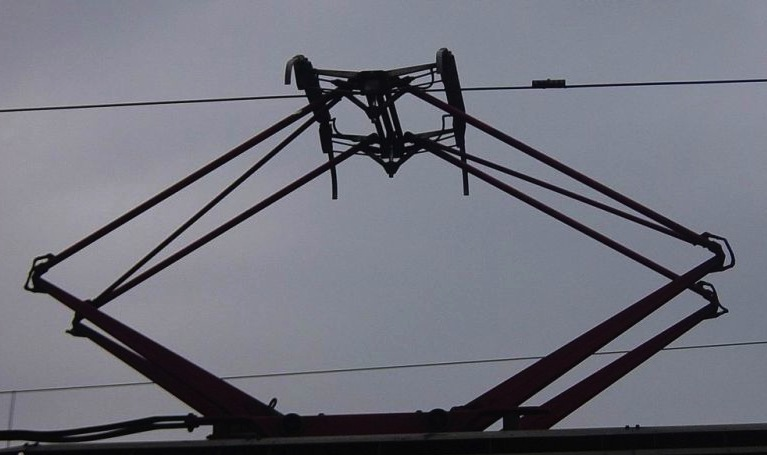
\includegraphics[width=.48\textwidth]{pantosimm}}\quad
%
\subfloat[][Architettura asimmetrica\label{fig:pantoinpresa-asimm}]
   {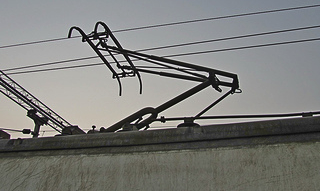
\includegraphics[width=.48\textwidth]{pantoinpresa2}}
%
\caption{Esempi di pantografi.}
%
\label{fig:pantoinpresa}
%
\end{figure}
%
% ------------------------------------------------------------------------ %
%
\subsubsection{Argomento da Approfondire1}
%
Qualche citazione \parencite{collina:2002:numerical-simulation-of-pantograph-overhead,comini:2008:fondamenti-di-termofluidodinamica-computazionale}.
%
\lipsum[1-3]
%

\bigskip

E adesso una nota a piè di pagina.\footnote{Nota a piè di pagina.}
In figura~\vref{fig:noimage} non è riportata alcuna immagine\dots o forse si?
%
% FIGURE
% ------------------------------------------------------------------------ %
% noimage
% ------------------------------------------------------------------------ %
%
\begin{figure}
%
\centering
%

\includegraphics[width=.6\textwidth]{noimage}
%
\caption{Nessuna immagine\dots Sorry.}
%
\label{fig:noimage}
%
\end{figure}
%
% ------------------------------------------------------------------------ %
%
\subsubsection{Scopi della Tesi}
%
\lipsum[1-3]
%
% ------------------------------------------------------------------------ %
%
\clearpage
%
\subsection*{Outline}
%
\par Il testo della tesi è così strutturato:
%
% ------------------------------------------------------------------------ %
%
\begin{description}
%
\item[{\hyperref[cap:statoarte]{Nel primo capitolo}}] è delineato lo stato dell'arte \lipsum[1]
%
\item[{\hyperref[cap:provesperimentali]{Il secondo capitolo}}] presenta i risultati della campagna di prove sperimentali \lipsum[2]
%
\item[{\hyperref[cap:analisinumeriche]{Nel terzo capitolo}}] si descrivono le scelte di modellazione \lipsum[3]
%
\end{description}
%
% ------------------------------------------------------------------------ %
%
\chapter{Focusing for X-rays}
\label{Introduzione}
\thispagestyle{empty}


Image formation by an optical system usually implies some form of focusing. Moreover the environment in which the radiation its surrounded, such as the material of which a certain mirror is made, controls the focusing property. In case of the visible light the focusing elements mainly used are lenses with their laws, well-known and studied, for the electron focusing, the optical element become electric and magnetic fields that to curve the path of the electrons. To study the focusing property of the X-ray radiation, it have to consider the interaction that acts between the radiation and the matter. These phenomena are, that rule the interaction radiation-matter are:
\begin{enumerate}
\item elastic scattering;
\item inelastic scattering;
\item absorption via photoelectric effect.
\end{enumerate}
The first effect, where there is an exchange of energy, is constituted by: Thomson scattering, that it is the scattering of electromagnetic radiation by a free non relativistic charged particle \cite{ThomsonScattering}, and Rayleigh scattering, an elastic scattering between the radiation and the strongly bounded electrons that act cooperatively \cite{RayleighScattering}. Because, the elastic scattering, generated a defned phase relation beetween the incident and the scattered radiation, it is the responsible of Bragg diffraction. The second effect ,inelastic scattering, or Compton scattering \cite{ComptonScattering}, that occurs when an electron lost by the atom interact with the radiation and absorb a small energy from the X-ray radiation. This scattering is an incoherent effect so there isn't any phase relation between incident and scattered radiation, moreover the atom pass to another quantum state due to the energy absorbed by the electron. The last effect, absorption via photoelectric effect, occur when an bounded electron with an atom get the necessary energy to break the bound and become free (ionization process). This last phenomenon is the most important effet fot the energies of interest at ESRF, i.e. $- keV $.
%
\begin{figure}[]
%
\centering
%
\subfloat[][$H_2 O $ \label{fig: Scattering1}]
   {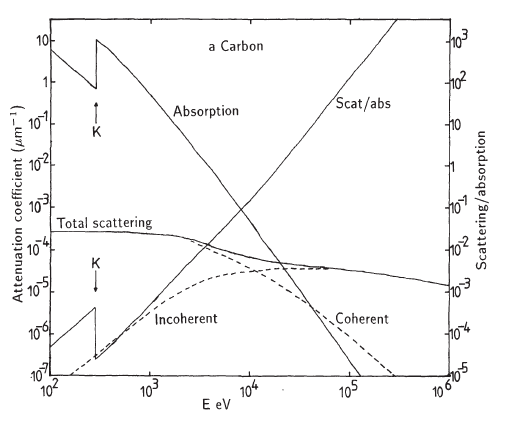
\includegraphics[width=.65\textwidth]{Immagini/Chapter1/Scattering1}}\quad
%
\subfloat[][$Pb $ \label{fig: Scattering2}]
   {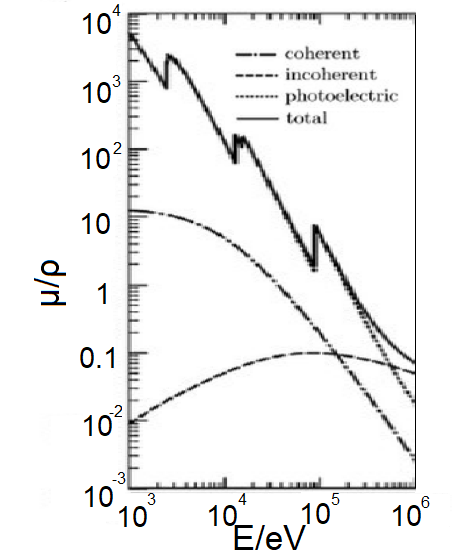
\includegraphics[width=.65\textwidth]{Immagini/Chapter1/Scattering2}}
%
\caption{Attenuation coefficient for X-ray radiation of a light material (water Figure \ref{fig: Scattering1}), and an heavy material (lead \ref{fig: Scattering2}) (from \cite{article_res_geat}).}
\label{fig :AttenuationCoefficient}
%
\end{figure}
Figure \ref{fig :AttenuationCoefficient} show the contribution for the attenuation coefficient, of the different absorption of a light material (water Figure \ref{fig: Scattering1}), and an heavi material (lead \ref{fig: Scattering2}) (from \cite{article_res_geat}.

\section{Interaction with Matter}
\label{sec: Interaction with Matter}
Interaction between radiation and matter can be compressed in an coefficient (absorption coefficient)), that rule the attenuation of an incident radiation

\begin{equation}
I = I_0 exp(-\mu x)
\label{eq: intensity}
\end{equation}

\begin{flushleft}
where $x $ is the thickness of the material, $\mu$ is the absorption coefficient, and $I_0$ the initial intensity of the beam corresponding to the intensity at $x=0$. Considering the beam as a plane wave, it is possible to express the  amplitude of the electromagnetic wave as:
\end{flushleft}

\begin{equation}
A=A_0exp(\frac{-2 \pi \beta x}{\lambda})exp(\frac{-2 \pi i ((1 - \delta)x-ct)}{\lambda})
\label{eq: amplitude}
\end{equation}

\begin{flushleft}
where $x$ is the position of the front wave, $\lambda$ correspond to the wavelength of the wave in the vacuum, $\delta $ is a number that describe the dispersive aspect of the wave-matter interaction, and $\beta $ is the absorption coefficient that describe the absorption aspect of the wave-matter interaction. The propagation of the radiation depend from the complex refractive index $n $, that can be expressed as: 
\end{flushleft}

\begin{equation}
n = 1 - \delta - i \beta
\label{eq: n_comlex}
\end{equation}

\begin{flushleft}
For X-rays process , the absorption term is the leading term, this mean that the $\mu$ coefficient can be defined as linearly dependent from the absorption coefficient, where:
\end{flushleft}

\begin{equation}
\alpha = \frac{4 \pi \beta}{\lambda}
\label{eq: alpha1}
\end{equation}

\begin{flushleft}
Normally the absorption values tabulated are given are the mass absorption coefficients $\mu_m$, where
\end{flushleft}

\begin{equation}
\mu = \mu_m \rho
\label{eq: alpha2}
\end{equation}

\begin{flushleft}
where $\rho $ is the density of the material. The mass absorption of a compound is given by
\end{flushleft}

\begin{equation}
\mu \textsubscript{m,com} = \sum_{j} w_j \mu_{m,j}
\label{eq: mu_com}
\end{equation}

\begin{flushleft}
where $\mu_{m,j} $ is the mass absorption of a particular element, and $w_j $ is the fraction of the $j $ element in the material. The relation between the absorption coefficient of the material and the mass absorption coefficient is:
\end{flushleft}

\begin{equation}
\alpha \textsubscript{com} = \mu \textsubscript{m,com} \rho \textsubscript{com}
\label{eq: alpha com}
\end{equation}

\begin{flushleft}
where $\rho \textsubscript{com}$ is the density of the compound.
\end{flushleft}

Because of the dominant energy of the radiation with respect to the matter energies involved in the interaction (X-rays energies spreads from 100eV, soft X-ray, to 10keV, hard X-ray, binding and molecular energies are of the order of few eV), the ionization process, as said before, is the leading process in the absorption coefficient. In this case the greater part of the energies involved is transferred to the kinetic term of the ionized electrons. Electron in atom have a well-defined state of energies, so, to be absorbed, the radiation must have at least an energy equal to an electron state energies. For energies equal to the electron state energies, as showed in Figure \ref{fig :AttenuationCoefficient}, absorption edges appears. The nomenclature $K,L,,M $, of those edges, that are not important for our treatment, correspond to, as it is showed in Figure \ref{fig: KLM}, the energies of an electron that goes down from a greater level, for example $n=2 $ to a lower one $n=1 $ (\cite{agarwal1991interaction}). In reality, the edges, are less pronunciation as the ones in figure, due to the finite energy width of the states, and because of the environment effect.
\\
\begin{figure}[]
%
\centering
%
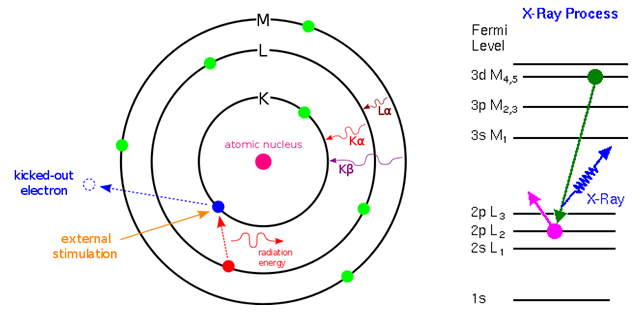
\includegraphics[width=.6\textwidth]{Immagini/Chapter1/KLM}
%
\caption{X-ray ionizing process}
%
\label{fig: KLM}
%
\end{figure}
To understand better the absorption of the X-ray radiation it is reported a brief theoretical treatment of the interaction, because the result are useful for the design of the optical element used for X-rays. The calculation start from the elastic scattering between  X-ray photon against free electron (Thomson scattering). The electro-magnetic radiation is characterized by an electric field with amplitude $A_0$ that accelerate a free electron (of charge $e $ and mass $m_e $) by an amount of $A_0 $($e / m $). A charged particle that is accelerated emits radiation, this change the value of the amplitude of the electric field equal to:

\begin{equation}
A_T(\Phi) = \frac{e}{4 \pi \epsilon_0 c^2 \vec{r}} \vec{a} \sin \Phi
\label{eq: At1}
\end{equation}

\begin{flushleft}
where $r $ is the distance from the charge, $\Phi $ correspond to the angle between the position vector \textbf{r} and acceleration vector \textbf{a}. Replacing \textbf{a} with $A_0 $($e / m $):
\end{flushleft}

\begin{equation}
A_T(\Phi) = A_0 \frac{e^2}{4 \pi \epsilon_0 c^2 \vec{r}} \sin \Phi
\label{eq: At2}
\end{equation}

\begin{flushleft}
To treat the interaction between the bounded electron and the radiation, going beyond the Thomson scattering, it is possible to multiply the Thomson amplitude $A_T (\Phi) $ to a complex number  is multiplied to a complex number $f = f_1 + if_2 $ named complex atomic scattering. Thus:
\end{flushleft}

\begin{equation}
A(\Phi, E) = A_t(\Phi) * f(E) = A_T(\Phi) [f_1(E) + if_2(E)]
\label{eq: A(fi, E)}
\end{equation}

\begin{flushleft}
where the two function $f_1 $ and $f_2 $, depend on the energy of the incident X-ray radiation that, to a first approximation, are independent from the angle between the incident and the scattered radiation $\theta $. This approximation has sense because the typical radiation length ($\sim 0.1-10nm $) is much larger than the typical length of the atomic electronic distribution ($\sim 1-50pm $), the consequence of this approximation is the possibility to consider a phase scattering of the atomic wave function. The values of the two function  $f_1 $ and $f_2 $ are calculated in the relativistic quantum dispersion theory \cite{cromer1970relativistic} and are given by:
\end{flushleft}

\begin{equation}
f_1(E) = Z + 4 \frac{\epsilon_0 m_e c}{h e^2} \int_{0}^{+ \infty}\frac{W^2 \sigma(W)}{E^2 - W^2} dW - \Delta_{rel}
\label{eq: f1}
\end{equation}

\begin{flushleft}
and
\end{flushleft}

\begin{equation}
f_2(E) = 2 \frac{\epsilon_0 m_e c}{h} E \sigma(E)
\label{eq: f2}
\end{equation}

\begin{flushleft}
In Equation \ref{eq: f1}, the first term correspond to the Thomson scattering, where $Z $ correspond to the atomic number of the atom. To add the angle-dependence of the scattering it is used the factor:
\end{flushleft}

\begin{equation}
f0 = \int_{0}^{+ \infty} U(r) sinc \left[ \frac{4 \pi r}{\lambda} \sin \frac{\theta}{2} \right] dr
\label{f0}
\end{equation}

\begin{flushleft}
where $U(r) $ represent the radial charge distribution and $sinc(x)$ is the cardinal sine function $ = \frac{\sin x}{x} $. Considering a wavelength $\lambda $ of the order of nanometres, if $\sin \frac{\theta}{2} \leq \frac{\lambda}{2}, f_0=Z $, otherwise for $\sin \frac{\theta}{2}=\lambda$, typically, for most element $ f_0 \simeq 0.9Z $.
\end{flushleft}
In Equation \ref{eq: f1}, the second term (the anomalous dispersion integral), represent the oscillation of the electron after the interaction with the radiation, this can be obtained treating the semi-classically the problem. This approach neglect the damping, so, near the absorption edges $f1 $ is inaccurate. The second term of the Equation \ref{eq: f1}, and in Equation \ref{eq: f2} contain $\sigma $ that is the photo ionization cross section expressed in $m^2 atom ^{-1} $, a coefficient that is related to the mass absorption coefficient in this way: 

\begin{equation}
\sigma(E) = A \frac{\mu}{N_0}
\label{eq: sigma}
\end{equation}

\begin{flushleft}
where $A $ is the atomic weight and $N_0 $ the Avogadro's number ($N_0 = 6.22  10^{23} particle mol^{-1}) $. The value of $\sigma(E) $ is theoretically obtained knowing the atomic wave function of the atom, so, only for hydrogen it possible to have the correct value, for all the other system, the calculation can be done with approximation methods that give some uncertainty on $\sigma(E) $, consequently on the value of $f_1 $ and $f_2 $.
\end{flushleft}
In Equation \ref{eq: f1} the third term take in account the relativistic effect. This correction is given by \cite{cromer1970relativistic}:
\begin{equation}
\Delta_{rel} = \frac{5}{3} \frac{|E_{tot}|}{m_e c^2} + \frac{Z}{2} \left( \frac{E}{m_e c^2} \right)^2
\label{eq: Delta_rel}
\end{equation}

\begin{flushleft}
where $|E_{tot} |$ is the modulus of the total energy of the atom (that is negative), moreover, this third term is the less relevant in Equation \ref{eq: f1}, for X-ray energies, so it is possible to neglect it in the calculation.
\\
For photo absorption event by an electron bounded to an atom, far from the absorption edges, a good approximation is to consider the solid state environment distorted by the ionization of the electrons , because, the most affected electrons are the outer ones. After some calculation, is possible to relate the factors $f_1 $ and $f_2 $ with the macroscopic parameters $n $ and $\beta $:
\end{flushleft}

\begin{equation}
\delta = 1 - n = \frac{e^2 \hbar^2}{2 \epsilon_0 m_e E^2} \overline{f_1}
\label{eq: delta}
\end{equation}

\begin{flushleft}
and
\end{flushleft}

\begin{equation}
\beta = \frac{e^2 \hbar^2}{2 \epsilon_0 m_e E^2} \overline{f_2}
\label{eq: beta}
\end{equation}

\begin{flushleft}
where $\overline{f_1} $ and $\overline{f_2} $ are defined as follow:
\end{flushleft}

\begin{equation}
\overline{f_1} = \sum_j N_j f_{1j} \qquad \overline{f_2} = \sum_j N_j f_{2j}
\label{f1, f2, mean}
\end{equation}

\begin{flushleft}
and represent the average scattering factor per unit volume, $N_j $ is the total number of the particular $j $ element per unit volume. Putting everything together Equation \ref{eq: delta}, apart near the absorption edges, can be expressed as:
\end{flushleft}

\begin{equation}
\delta = \frac{N e^2 \hbar^2}{2 \epsilon_0 m_e  E^2} \overline{f_1}  = \frac{N e^2 \lambda^2}{8 \pi^2 \epsilon_0 m_e c^2} \overline{f_1}
\label{eq: delta new}
\end{equation}

\begin{flushleft}
where $N $ is the number of electrons per unit volume. For X-ray energies the value of $\delta $ is small (typically $\sim 10^{-3} $) and positive, this is important because it means that, for X-rays, the refractive index is a bit less than $1 $. It is possible to find the tabulated values of $f_1 $ and $f_2 $, \cite{henke1981atomic}, that are the main ingredient to calculate the curve in Figure \ref{fig :AttenuationCoefficient}  and these were used to generate Figure 1. This values, according with the experimental results, allow to write, far from absorption edges, the absorption coefficient $\beta $ such as:
\end{flushleft}

\begin{equation}
\beta \sim Z^2 \lambda^3
\label{eq: new beta}
\end{equation}

\begin{flushleft}
This mean that increasing the photon energy, the absorption decrease, and is it consistent with Figure \ref{fig :AttenuationCoefficient}, far from the edges. Moreover, the absorption, become bigger with the element used in the optical element, heavy elements absorb more than light elements. This is the reason why, to use refractive lenses for x-ray radiation, one of the used material is the Beryllium.
\end{flushleft}


\section{Total External Reflection}
\label{sec: Total Externa Reflection}
\begin{flushleft}
For the system in Figure \ref{fig: System}, there are two complex refractive index:
\end{flushleft}
\begin{equation}
\overline{n_1} = 1 - \delta_1 - i \beta_1 = n_1 - i \beta_1
\label{eq: n1}
\end{equation}
and
\begin{equation}
\overline{n_2} = 1 - \delta_2 - i \beta_2 = n_2 - i \beta_2
\label{eq: n1}
\end{equation}
\begin{flushleft}
moreover $\delta_2 > \delta_1 $. In the general case there are, as shown in Figure \ref{fig: System} a reflected and a transmitted wave. For the theoretical treatment, initially, will be neglect the absorption ($\beta_1 = \beta_2 = 0$), moreover the permeability coefficient it is supposed to be similar to the permeability in the vacuum. Thus, the law of Snell, can be expressed such as: 
\end{flushleft}
\begin{equation}
\frac{\cos \theta_i}{\cos \theta_t} = \frac{1 - \delta_2}{1 - \delta_1}
\label{eq: snell 1}
\end{equation}
\begin{figure}[]
%
\centering
%
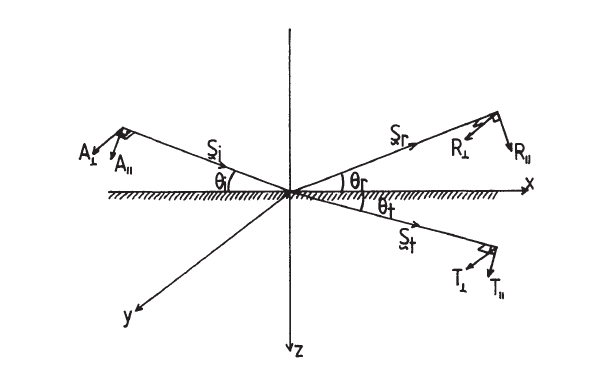
\includegraphics[width=.6\textwidth]{Immagini/Chapter1/System}
%
\caption{Interface of two medium}
%
\label{fig: System}
%
\end{figure}
\begin{flushleft}
Using the frame system as in Figure \ref{fig: System}, with the z-axis that correspond to the normal of the interface. It is possible to write the component of the electric field of the waves in this way
\end{flushleft}
\begin{subequations}
\begin{equation}
E_{ix} = A_{\parallel} \sin \theta_i \exp^{- i \tau_i}, \hspace{4mm}
E_{iy} = A_{\perp} \exp^{- i \tau_i}, \hspace{4mm} 
E_{iz} = A_{\parallel} \cos \theta_i \exp^{- i \tau_i}
\label{eq: E component 1}
\end{equation}
\begin{equation}
E_{tx} = - T_{\parallel} \sin \theta_t \exp^{- i \tau_t}, \hspace{4mm}
E_{ty} = T_{\perp} \exp^{- i \tau_t}, \hspace{4mm} 
E_{tz} = T_{\parallel} \cos \theta_t \exp^{- i \tau_t}
\label{eq: E component 2}
\end{equation}
\begin{equation}
E_{rx} = R_{\parallel} \sin \theta_r \exp^{- i \tau_r}, \hspace{4mm}
E_{ry} = R_{\perp} \exp^{- i \tau_r}, \hspace{4mm} 
E_{rz} = R_{\parallel} \cos \theta_r \exp^{- i \tau_r}
\label{eq: E component 3}
\end{equation}
\end{subequations}
\noindent  where
\begin{subequations}
\begin{equation}
\tau_i = \omega ( t - \frac{\vec{r} \bullet \vec{s_i} }{v_1}) = \omega \left[ t - \frac{(1 - \delta_1 ) ( x \cos \theta_i + z \sin \theta_i}{c} \right]
\label{eq: tau 1}
\end{equation}
\begin{equation}
\tau_t = \omega ( t - \frac{\vec{r} \bullet \vec{s_t} }{v_2}) = \omega \left[ t - \frac{(1 - \delta_2 ) ( x \cos \theta_t + z \sin \theta_t}{c} \right]
\label{eq: tau 2}
\end{equation}
\begin{equation}
\tau_r = \omega ( t - \frac{ \vec{r} \bullet \vec{s_r} }{v_1}) = \omega \left[ t - \frac{(1 - \delta_1 ) ( x \cos \theta_r + z \sin \theta_r}{c} \right]
\label{eq: tau 3}
\end{equation}
\end{subequations}
\begin{flushleft}
where $\omega $ is the angular frequency of the wave, and $v_1, v_2 $, correspond to the velocities of propagation that depend on the material as follow:
\end{flushleft}
\begin{equation}
v_1 = \frac{c}{1 - \delta_1}, \hspace{4mm} v_2 = \frac{c}{1 - \delta_2}
\end{equation}
\begin{flushleft}
the related magnetic field are:
\end{flushleft}
\begin{subequations}
\begin{equation}
\begin{aligned}
H_{ix} = - A_{\perp} (1 - \delta_1) \sin \theta_i \exp^{-i \tau_i}, \hspace{4mm}
H_{iy} = - A_{\parallel} (1 - \delta_1) \exp^{-i \tau_i}, \\
H_{iz} =  A_{\perp} (1 - \delta_1) \cos \theta_i \exp^{-i \tau_i}
\end{aligned}
\label{eq: H1}
\end{equation}
\begin{equation}
\begin{aligned}
H_{tx} = - T_{\perp} (1 - \delta_2) \sin \theta_t \exp^{-i \tau_t}, \hspace{4mm}
H_{ty} = - T_{\parallel} (1 - \delta_2) \exp^{-i \tau_t}, \\
H_{tz} =  T_{\perp} (1 - \delta_2) \cos \theta_t \exp^{-i \tau_t}
\end{aligned}
\label{eq: H2}
\end{equation}
\begin{equation}
\begin{aligned}
H_{rx} = - R_{\perp} (1 - \delta_1) \sin \theta_r \exp^{-i \tau_r}, \hspace{4mm}
H_{ry} = - R_{\parallel} (1 - \delta_1) \exp^{-i \tau_r}, \\
H_{rz} =  R_{\perp} (1 - \delta_1) \cos \theta_r \exp^{-i \tau_r}
\label{eq: H3}
\end{aligned}
\end{equation}
\end{subequations}
\begin{flushleft}
the boundary condition impose the continuity of the fields:
\end{flushleft}
\begin{equation}
E_{ix} + E_{rx} = E_{tx}, \hspace{4mm} E_{iy} + E_{ry} = E_{ty}
\label{eq: continuity E}
\end{equation}
\noindent and
\begin{equation}
H_{ix} + H_{rx} = H_{tx}, \hspace{4mm} H_{iy} + H_{ry} = H_{ty}
\label{eq: continuity H}
\end{equation}
\begin{flushleft}
because of Snell's laws $\theta_r = \theta_t $, so, from the Equation \ref{eq: continuity E} and Equation \ref{eq: continuity H}:
\end{flushleft}
\begin{subequations}
\begin{equation}
(A_{\parallel} - R_{\parallel}) \sin \theta_i = T_{\parallel} \sin_t
\label{eq: mix1}
\end{equation}
\begin{equation}
A_{\perp} + R_{\perp} = T_{\perp}
\label{eq: mix2}
\end{equation}
\begin{equation}
(1 - \delta_1 ) (A_{\perp} - R_{\perp}) \sin \theta_i = (1 - \delta_2) T_{\perp} \sin \theta_t
\label{eq: mix3}
\end{equation}
\begin{equation}
(1 - \delta_1) (A_{\parallel} +R_{\parallel}) = (1 - \delta_2) T_{\parallel}
\label{eq: mix4}
\end{equation}
\label{eq: mix}
\end{subequations}
\begin{flushleft}
Equations \ref{eq: mix} give a set of equations where the parallel and perpendicular component of the waves are independent. Solving that set with respect to each parallel/perpendicular component it is obtained:
\end{flushleft}
\begin{subequations}
\begin{equation}
\begin{aligned}
\frac{R_{\parallel}}{A_{\parallel}} = \left[\frac{(1 - \delta_2) \sin \theta_i - (1 - \delta_1) \sin \theta_t}{(1 - \delta_2) \sin \theta_i} + (1 - \delta_1) \sin \theta_t \right]
\end{aligned}
\label{eq: R/A parll}
\end{equation}
\begin{equation}
\begin{aligned}
\frac{R_{\perp}}{A_{\perp}} = \left[\frac{(1 - \delta_1) \sin \theta_i - (1 - \delta_2) \sin \theta_t}{(1 - \delta_1) \sin \theta_i} + (1 - \delta_2) \sin \theta_t \right]
\end{aligned}
\label{eq: R/A perp}
\end{equation}
\begin{equation}
\begin{aligned}
\frac{T_{\parallel}}{A_{\parallel}} = \frac{2(1 - \delta_1) \sin \theta_i}{(1 - \delta_2) \sin \theta_i + (1 - \delta_1) \sin \theta_t}
\end{aligned}
\label{eq: T/A parll}
\end{equation}
\begin{equation}
\begin{aligned}
\frac{T_{\perp}}{A_{\perp}} = \frac{2(1 - \delta_1) \sin \theta_i}{(1 - \delta_1) \sin \theta_i + (1 - \delta_2) \sin \theta_t}
\end{aligned}
\label{eq: T/A perp}
\end{equation}
\label{eq: parall and perp 1}
\end{subequations}
\begin{flushleft}
Equations \ref{eq: parall and perp 1} are the \textbf{Fresnel formula} for reflection at a plane surface. Combining them with Equation \ref{eq: snell 1} it is obtained:
\end{flushleft}
\begin{subequations}
\begin{equation}
\begin{aligned}
\frac{R_{\parallel}}{A_{\parallel}} = \frac{(1 - \delta_2)^2 \sin \theta_i - (1 - \delta_1) \sqrt{(1 - \delta_2)^2 - (1 - \delta_1)^2 \cos^2 \theta_i}}{(1 - \delta_2)^2 \sin \theta_i +  (1 - \delta_1) \sqrt{(1 - \delta_2)^2 - (1 - \delta_1)^2 \cos^2 \theta_i}} 
\end{aligned}
\label{eq: R/A parll 1}
\end{equation}
\begin{equation}
\begin{aligned}
\frac{R_{\perp}}{A_{\perp}} = \frac{(1 - \delta_1)^2 \sin \theta_i - \sqrt{(1 - \delta_2)^2 - (1 - \delta_1)^2 \cos^2 \theta_i}}{(1 - \delta_1)^2 \sin \theta_i  +  \sqrt{(1 - \delta_2)^2 - (1 - \delta_1)^2 \cos^2 \theta_i}} 
\end{aligned}
\label{eq: R/A perp 1}
\end{equation}
\begin{equation}
\begin{aligned}
\frac{T_{\parallel}}{A_{\parallel}} = \frac{2(1 - \delta_1) (1 - \delta_2) \sin \theta_i }{(1 - \delta_2)^2 \sin \theta_i  +  (1 - \delta_2)\sqrt{(1 - \delta_2)^2 - (1 - \delta_1)^2 \cos^2 \theta_i}} 
\end{aligned}
\label{eq: T/A parll 1}
\end{equation}
\begin{equation}
\begin{aligned}
\frac{T_{\perp}}{A_{\perp}} = \frac{2(1 - \delta_1) \sin \theta_i }{(1 - \delta_1) \sin \theta_i  +  \sqrt{(1 - \delta_2)^2 - (1 - \delta_1)^2 \cos^2 \theta_i}} 
\end{aligned}
\label{eq: T/A perp 1}
\end{equation}
\label{eq: parall and per 2}
\end{subequations}
\begin{flushleft}
When $\theta_i $ is such that:
\end{flushleft}
\begin{equation}
\cos \theta_c = \frac{1 - \delta_2}{1 - \delta_1}
\label{eq: theta_c}
\end{equation}
\begin{flushleft}
that angle is named critical angle $\theta_c $, and
\end{flushleft}
\begin{equation}
\frac{R_{\parallel}}{A_{\parallel}} = \frac{R_{\perp}}{A_{\perp}}
\label{eq: R/A critical}
\end{equation}
\begin{flushleft}
this case correspond to a wave that is totally reflected. Normally the total external reflection take place at an interface light material(air/vacuum) and dense material, so $\delta_1 = 0, \delta_2 = \delta$, the equations became:
\end{flushleft}
\begin{equation}
\cos \theta_c = 1 - \delta \qquad for \hspace{2mm} small \hspace{2mm} angle \qquad \theta_c \simeq \sqrt{2 \delta}
\end{equation}
\begin{flushleft}
and:
\end{flushleft}
\begin{subequations}
\begin{equation}
\begin{aligned}
\frac{R_{\parallel}}{A_{\parallel}} = \frac{(1 - \delta)^2 \sin \theta_i - \sqrt{(1 - \delta)^2 - \cos^2 \theta_i}}{(1 - \delta)^2 \sin \theta_i + \sqrt{(1 - \delta_2)^2 - \cos^2 \theta_i}} 
\end{aligned}
\label{eq: R/A parll 2}
\end{equation}
\begin{equation}
\begin{aligned}
\frac{R_{\perp}}{A_{\perp}} = \frac{\sin \theta_i - \sqrt{(1 - \delta)^2 - (1 - \cos^2 \theta_i}}{\sin \theta_i  +  \sqrt{(1 - \delta)^2 - \cos^2 \theta_i}} 
\end{aligned}
\label{eq: R/A perp 2}
\end{equation}
\begin{equation}
\begin{aligned}
\frac{T_{\parallel}}{A_{\parallel}} = \frac{2(1 - \delta) \sin \theta_i }{(1 - \delta)^2 \sin \theta_i  +  \sqrt{(1 - \delta)^2 - (1 - \cos^2 \theta_i}} 
\end{aligned}
\label{eq: T/A parll 2}
\end{equation}
\begin{equation}
\begin{aligned}
\frac{T_{\perp}}{A_{\perp}} = \frac{2 \sin \theta_i }{ \sin \theta_i  +  \sqrt{(1 - \delta)^2 - \cos^2 \theta_i}} 
\end{aligned}
\label{eq: T/A perp 2}
\end{equation}
\label{eq: parall and per 3}
\end{subequations}
\begin{flushleft}
introducing the absorbing coefficient $\beta_2 = \beta \neq 0 $:
\end{flushleft}
\begin{subequations}
\begin{equation}
\begin{aligned}
\frac{R_{\parallel}}{A_{\parallel}} = \frac{\overline{n}^2 \sin \theta_i - \sqrt{\overline{n}^2 - \cos^2 \theta_i}}{\overline{n}^2 \sin \theta_i + \sqrt{\overline{n}^2 - \cos^2 \theta_i}} 
\end{aligned}
\label{eq: R/A parll 3}
\end{equation}
\begin{equation}
\begin{aligned}
\frac{R_{\perp}}{A_{\perp}} = \frac{\sin \theta_i - \sqrt{\overline{n}^2 - \cos^2 \theta_i}}{(\sin \theta_i  +  \sqrt{\overline{n}^2 - \cos^2 \theta_i}} 
\end{aligned}
\label{eq: R/A perp 3}
\end{equation}
\begin{equation}
\begin{aligned}
\frac{T_{\parallel}}{A_{\parallel}} = \frac{2\overline{n} \sin \theta_i }{\overline{n}^2 \sin \theta_i  +  \sqrt{\overline{n}^2 - \cos^2 \theta_i}} 
\end{aligned}
\label{eq: T/A parll 3}
\end{equation}
\begin{equation}
\begin{aligned}
\frac{T_{\perp}}{A_{\perp}} = \frac{2 \sin \theta_i }{ \sin \theta_i  +  \sqrt{\overline{n}^2 - \cos^2 \theta_i}} 
\end{aligned}
\label{eq: T/A perp 3}
\end{equation}
\label{eq: parall and per 4}
\end{subequations}
For interface that are curved, the Equations \ref{eq: parall and per 4} are still valid if the curvature radius is much grater that the wavelength, condition that is satisfied for the X-ray radiation.
The reflectivity are defined in these way::
\begin{equation}
R_p =\frac{R_{\parallel}}{A_{\parallel}} \left(\frac{R_{\parallel}}{A_{\parallel}} \right)^{*}
\label{eq: Rp}
\end{equation}
\noindent and
\begin{equation}
R_p =\frac{R_{\parallel}}{A_{\parallel}} \left(\frac{R_{\parallel}}{A_{\parallel}} \right)^{*}
\label{eq: Rs}
\end{equation}
\begin{flushleft}
Figure \ref{fig: IdealReflection}, show the behaviour of an ideal non absorbing material ($\beta = 0 $), where the reflection maintain its initial value up to the critical angle, and after fall down, in a way ruled by the dispersion coefficient $\delta $ which depend on the energy. In reality $\beta $ is never zero, so it is not possible to have total external reflection in the way defined before. It is convenient to define that the total external appear when there is  a point of inflection in the reflection curve with respect to the incidence angle $\theta_i $, this occurs when:
\end{flushleft}
\begin{equation}
\beta < 0.63 \delta
\label{eq: last}
\end{equation}
\begin{flushleft}
In Figure \ref{fig : Plottts} are plotted the reflectivity trend of three material (Si, Rh, Pb) with respect to the incidence angle, fixing the energy of the radiation at $5000 eV$, on a silicon substrate. As it is figured there is a  better behaviour, in sense of critical angle, for the light element because of them minor absorption coefficient $\beta $. This dependant mirror reflectivity is not implemented in my python library MONWES (but it could be done). 
\end{flushleft}
\begin{figure}[]
%
\centering
%
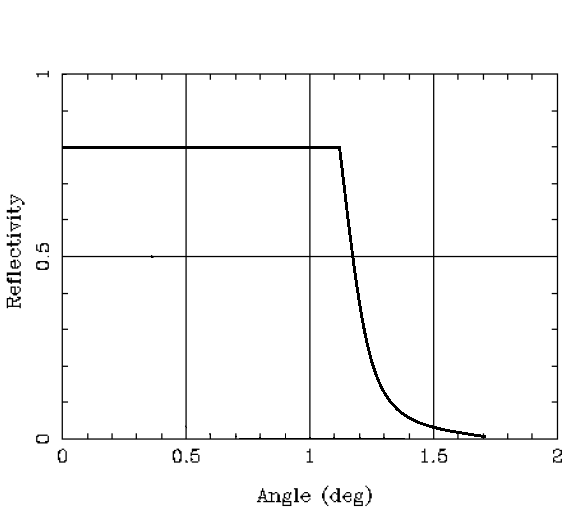
\includegraphics[width=.6\textwidth]{Immagini/Chapter1/IdealReflection}
%
\caption{Reflectivity for the case of a non-absorbing material}
%
\label{fig: IdealReflection}
%
\end{figure}
\begin{figure}[]
%
\centering
%
\subfloat[][Si  \label{fig: Si}]
   {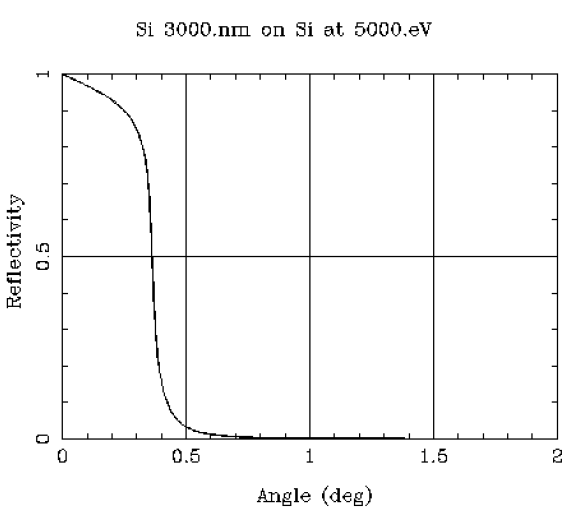
\includegraphics[width=.55\textwidth]{Immagini/Chapter1/Si}}
%
\subfloat[][Rh \label{fig: Rh}]
   {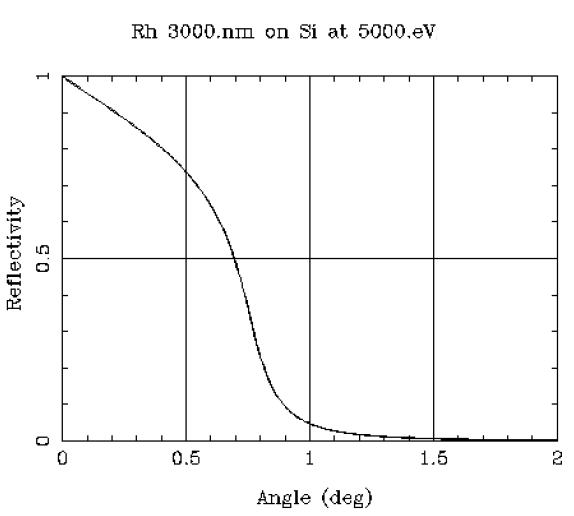
\includegraphics[width=.55\textwidth]{Immagini/Chapter1/Rh}}\quad
%
\subfloat[][Pb  \label{fig: Si}]
   {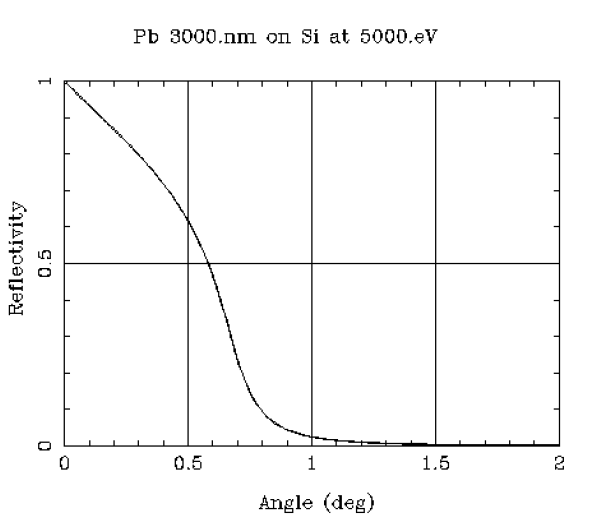
\includegraphics[width=.55\textwidth]{Immagini/Chapter1/Pb}}
%
\caption{Reflectivity plot with respect of the grazing incidence angle $\theta_i $ of different material with a radiation of $500 eV$ on a substrate of Si \cite{CXRO}}
\label{fig : Plottts}
%
\end{figure}
%
\chapter{Mirrors for X-rays}
\label{capitolo2}
\thispagestyle{empty}

\begin{quotation}
{\footnotesize
\noindent{\emph{``Terence: Tu lo reggi il whisky? \\
Bud: Beh, i primi due galloni si, al terzo divento nostalgico e ci pu\`o scappare la lite... E tu lo reggi? \\
Terence: Eh, che domande, io sono stato allattato a whisky!''
} }
\begin{flushright}
I due superpiedi quasi piatti
\end{flushright}
}
\end{quotation}
\vspace{0.5cm}

\noindent As discussed in Chapter \ref{capitolo1}, to have focusing properties for X-ray radiation, refraction optics are useless, due to the strong interaction with matter of X-rays. Thus reflection optics, at grazing incidence angle to have a good signal is needed. Mirrors that carry out any focusing must have a curved surface. A Working at normal incidence, it is possible to obtain a form a good image using a concave mirror. But this is not the case for X-ray that work, as said before, at grazing angle, this introduce some kind of optical aberration.A spherical surface has the property that the rate of change of the surface slope is exactly the same everywhere on the surface, and thus the aberration is inevitable. This shape bring an intrinsic aberration ("spherical aberration").
If the slope in not any more constant all over the mirror but become flatten in the region surrounding the outer rays, it is possible to focus all the rays in the same point. While correction of spherical aberration is not the only application of aspherical surfaces, it is one of the major application areas.

\section{Spherical surface}
\noindent To define a spherical surface is needed only the radius of curvature.  A spherical surface is defined by only one parameter, the radius of curvature of the surface. 
\subsection{Astigmatism}
In Figure \ref{fig: System1} it is showd an image formation of a beam with a spherical mirror with radius $R $, at grazing incidence $\theta_i $, with a divergence $\beta $ from the point source P. The oject length $u $ is equal to the distance PO and the image distance $v $ correspond to OQ.
\begin{figure}[]
%
\centering
%
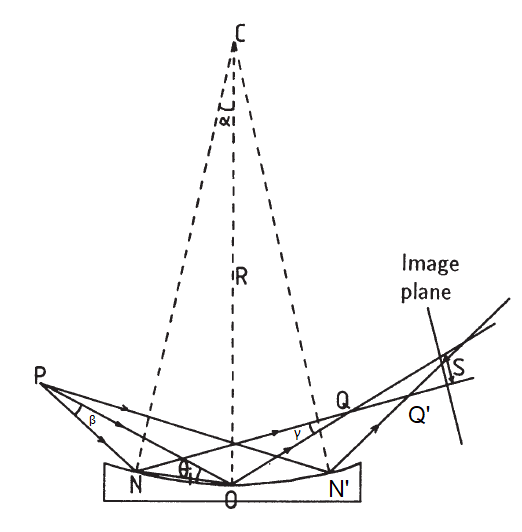
\includegraphics[width=.6\textwidth]{Immagini/Chapter2/System1}
%
\caption{Formation image of a circular mirror}
%
\label{fig: System1}
%
\end{figure}
\noindent The beam hit the mirror over a distance equal to $k = $ NO, such as $k<<R $, that correspond to a small divergence $\beta $. The cord NO subtends an angle $\alpha $ with the center of the sphere C, thus $k = R \alpha $, $\gamma $ is the convergence angle of the beam at the focal point Q. For small angle approximation, from the triangle PNO ,
\begin{equation}
\beta = R \alpha \frac{\theta_i - \alpha / 2}{u - R \alpha}
\label{eq: beta}
\end{equation}
\noindent and from QNO
\begin{equation}
\gamma = R \alpha \frac{\theta_i + \alpha / 2}{v + R \alpha}
\label{eq: gamme}
\end{equation}
\noindent The reflection law impose that $\beta + \gamma = 2 \alpha$, thus:
\begin{equation}
\frac{1 - \alpha / (2 \theta_i)}{u - R \alpha} + \frac{1 + \alpha / (2 \theta_i)}{v + R \alpha} = \frac{2}{R \theta_i}
\label{eq: refle lae}
\end{equation}
\noindent in case of paraxial approximation
\begin{equation}
\frac{1}{u} + \frac{1}{v} = \frac{2}{R \theta_i} = \frac{1}{f_m}
\label{eq: reflection law}
\end{equation}
\noindent where
\begin{equation}
f_m = \frac{R \sin \theta_i}{2}
\label{eq: fm}
\end{equation}
\noindent that it reduce to $f_m = \frac{R \theta_i}{2} $ for small angle, $f_m $ is named meridian focal length. 
\\
In case of a three dimensional spherical mirror, a second image is generated, as it is showed if Figure \ref{fig: MeridianAndSagittal},with a focal distance equal to:
\begin{equation}
f_s = \frac{R}{2 \sin \theta_i}
\label{eq: fs}
\end{equation}
\noindent and it is named sagittal focal length.
\begin{figure}[]
%
\centering
%
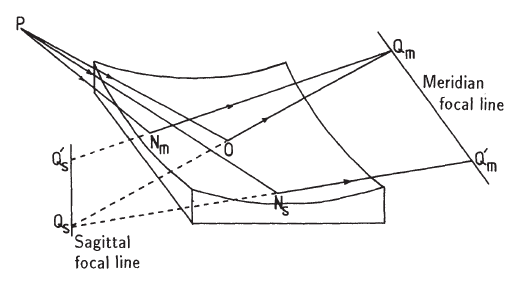
\includegraphics[width=.6\textwidth]{Immagini/Chapter2/MeridianAndSagittal}
%
\caption{Image formation of a 3D spherical mirror}
%
\label{fig: MeridianAndSagittal}
%
\end{figure}
\noindent For Figure \ref{fig: MeridianAndSagittal} it is possible to note that the two image for a point wise source are lines, where the meridial line is in the plane of the mirror and the sagittal line perpendicular to it. Equation \ref{eq: fm} and Equation \ref{eq: fs}, are equal for incidence angle $\theta_i = 0^{\circ} $ . In the case of grazing incidence the situation is bad, for example, with a $\theta_i = 2^{\circ} $, the sagittal focal length is $10^3$ times the meridial length.
\subsection{Spherical Aberration}
Spherical mirror are also affected, as it is showed in Figure \ref{fig: System1}, by a transverse spherical aberration. This aberration can be determined relating it with the the variation of $v $ with $\alpha$:
\begin{equation}
S = \Delta v \sin \gamma \simeq \Delta v \gamma
\label{eq: S}
\end{equation}
\noindent where S is the coefficient that determine the spherical aberration. Moreover, from Equation \ref{eq: refle lae}, in case of $\alpha =0 $:
\begin{equation}
v_0 = \frac{f_m u}{u - f}
\label{eq: v0}
\end{equation}
\noindent otherwise:
\begin{equation}
v = v_0 + \Delta v = f_m u - \frac {\frac{3 u R \alpha}{4} + \frac{R^2 \alpha^2}{2}}{u - \frac{3 R_{\alpha}}{4} - f_m}
\label{eq: v}
\end{equation}
\noindent defining a magnification such as
\begin{equation}
M = \frac{v}{u}
\label{eq: M}
\end{equation}
\noindent combining it with Equation \ref{eq: beta} and Equation \ref{eq: gamme}
\begin{equation}
\gamma = \frac{2 \alpha}{M + 1}
\label{eq: new gamme}
\end{equation}
\noindent So
\begin{equation}
S = \frac{3 R \alpha^2}{2} (M + 1) = \frac{3 k^2}{2 R} (M + 1)
\label{eq: new S}
\end{equation}
\noindent the dependance of S with respect to k is quadratic, so all the rays are deviated to the same side of $\alpha = 0$ image point.
\subsection{Reducing aberration}
For spherical mirror it is possible to reduce the aberration using large grazing angle (decrease astigmatism) and small aperture (decrease spherical aberration). For the first solution it have to consider the total external reflection, so it have to choose a material that have a big value of the critical angle $\theta_c $. An example can be the Carbon that have a critical angle of $\theta_c = 18^{\circ} $ for $K_{\alpha} $ radiation, this correspond to have a ratio $f_s $ over $f_m $ of $11 $, that is still big.
\\
Reducing the aperture it means to reduce $k $, it is reduce also the spherical aberration but also the collecting power of the mirror. This is bad because the resolving power is limited by the diffraction limit that is $\simeq \frac{\lambda}{2 \theta} $, where $\theta $ is the maximum semiaperture, that, for grazing angle, correspond to $\theta_i $.

\section{Conic Surfaces}
As said before, to go beyond the spherical mirror correcting the aberration, there exist aspherical surfaces that are defined with more than one parameter, in general by an analytical formula. The easier aspherical surface is the toroidal surface, a surface that is defined with two radii of curvature, the meridian one $R_m $ and the sagittal one $R_s $. A particular choice of radii can be
\begin{equation}
R_m \sin \theta_i = \frac{R_s}{\theta_i}
\label{eq: toroidal 1}
\end{equation}
\noindent in such a way to have equal focal length and so no asytgmatism. Thus
\begin{equation}
R_s = R_m \sin^2 \theta_i
\end{equation}
Other kind of aspherical surfaces are those named $"conic surfaces"$ that can be defined as

\begin{equation}
	z = \frac{c r^2}{1 + \sqrt{1 - (1 + k)} c^2 r^2}
\end{equation}

\noindent where $c $ is the base curvature at the vertex, $k $ is a constant that define the kind of conical surface, and $r $ is the radial coordinate of the point on the surface. In Table \ref{tab: conic surface}, and in Figure \ref{fig: SurfaceConic1} is showed the relation between the $k $ constant and the kind of surface

\begin{table}[ht]
	\centering
		\begin{tabular}{l|r}
			Conic Constant k & Surface Type\\
			\hline
			0 & Sphere \\
			$k < -1 $ & Hyperboloid \\
			$k = -1 $ & Paraboloid \\
			$-1 < k < -0 $ & Ellipsoid \\
			$k > 0 $ & Oblate Ellipsoid \\	
		\end{tabular}
	\caption{Parameter of different conic surfaces}
	\label{tab: conic surface}
\end{table}
\begin{figure}[]
%
\centering
%
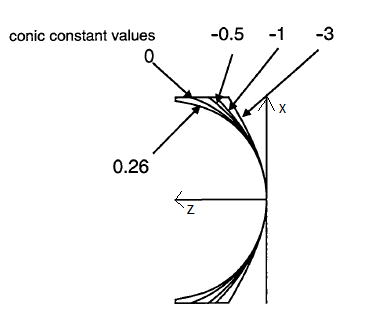
\includegraphics[width=.4\textwidth]{Immagini/Chapter2/SurfaceConic1}
%
\caption{Different kind of surface conic, with the same $c $ base curvature value, and different constant $k $.}
%
\label{fig: SurfaceConic1}
%
\end{figure}
\noindent A good point that have the conical surfaces are the no-presence of spherical aberration. As said in before, spherical surface affected buy spherical aberration if the configuration is different from the normal incidence. The ellipsoidal geometry forms create a free-aberration image for a couple of real object on the same side of the surface, on the contrary the hyperbola work for conjugates on different side of it. Parabolic surface create a perfect image for any axial object place at infinity, this is the reason why parabolic mirror are very used for astronomical application. For all the shapes of surfaces, if the object is moved from it's ideal position aberration will appear: an axial movement introduce a certain amount of spherical aberration, lateral movement introduce other types of aberration such as coma, astigmatism and field curvature.
\\
\noindent The importance of aspherical surface for mirror consist in the fact that, differently from the lenses, is not possible to build a spherical surface with different radii, in the lenses case it different spherical radii, and so, aspherical surface, serve to minimize the aberration. 
Figure \ref{fig :spher abb corr} show a simple example of how it is possible to correct the spherical aberration using a paraboloid mirror \ref{fig: ParabolicMirror} instead of a spherical mirror \ref{fig: Sphericalmirror}
\begin{figure}[]
%
\centering
%
\subfloat[][Spherical mirror \label{fig: Sphericalmirror}]
   {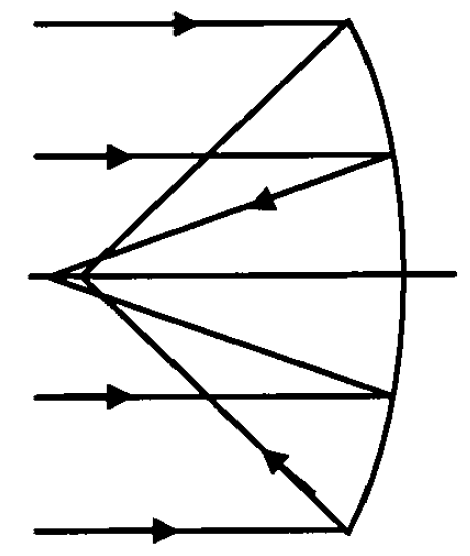
\includegraphics[width=.2\textwidth]{Immagini/Chapter2/SphericalMirror}}\quad
%
\subfloat[][Parabolic Mirror  \label{fig: ParabolicMirror}]
   {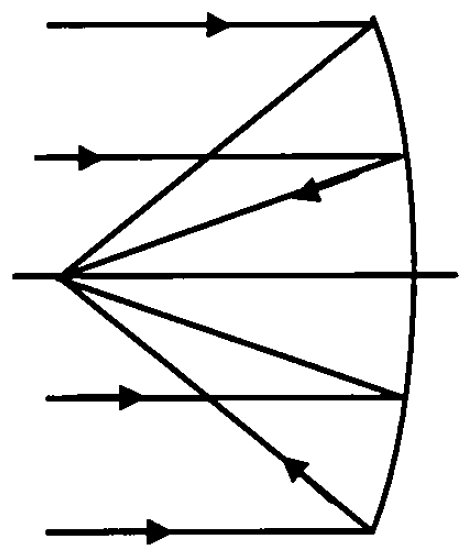
\includegraphics[width=.2\textwidth]{Immagini/Chapter2/ParabolicMirror}}
%
\caption{Example of spherical aberration correction}
\label{fig :spher abb corr}
%
\end{figure}

\section{Compound Optical system}
An optical system designed to obtain an image that reproduce correctly the object image must satisfy the Sine-Abbe condition
\begin{equation}
\frac{sin u^{'}}{sin U^{'}} = \frac{sin u}{ sin U}
\label{eq: SineAbbe}
\end{equation} 
\noindent where, as it is showed in Figure \ref{fig: SineAbbe}, $u $ and $u^{'} $ are rays that leave the object, $U$ and $U^{'} $ are the angles of the same rays that reach the image plane. In other world, the sine of the ray that leave the object must be proportional to the sine of the angles that reach the image plane.
\begin{figure}[]
%
\centering
%
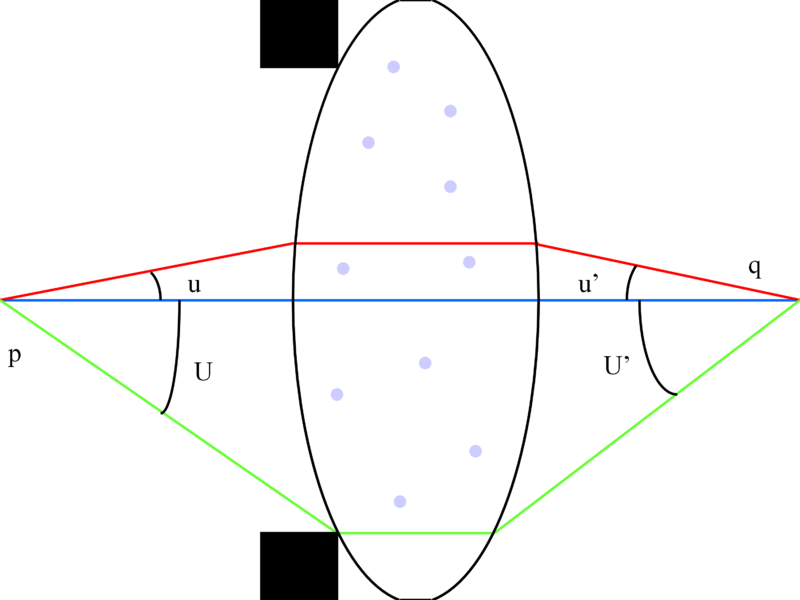
\includegraphics[width=.6\textwidth]{Immagini/Chapter2/SineAbbeCondition}
%
\caption{Sine Abbe condition for a lens}
%
\label{fig: SineAbbe}
%
\end{figure}
Unfortunately, for the case of mirror, there is no way to satisfy the Sine Abbe condition using only one mirror. To satisfy the condition, and so obtain a better image, there are invented optical system composed by more than one mirror. The system that whose invented which respect the condition are the Wolter system, widely used in astronomy, that use a combination of coaxial and confocal conic section.A first approximation system that respect the sine Abbe condition are the Kirkpatrick-Baez system and Montel or nested-Kirkpatrik-Baez system, those compound optical system involves reflector whose meridian planes are at right angle (crossed).
\subsection{Wolter System}
\hspace{10mm} In 1952 Wolter published a paper in which he discussed several disposition of two conical mirror in order to collect light for an astronoical use. Figure show the different disposition discussed: Wolter $\mathrm{I} $, Wolter $\mathrm{II} $, Wolter $\mathrm{III} $.
\noindent Wolter $\mathrm{I} $ telescope consist of a coaxialparaboloid (primary mirror) and hyperboloid (secondary mirror). The focus of the paraboloid is coincident with the rear focus of the hyperboloid, and the reflection inside both mirrors. The Wolter $\mathrm{II} $ telescope use the same kind of mirror of Wolter $\mathrm{I} $ paraboloid and hyperboloid. But the focus of the paraboloid coincident with the front focus of the hyperboloid, and, the reflection, occurs internally for the paraboloid and externally for the hyperboloid. The Wolter $\mathrm{III} $ telescope consist in a paraboloid and an ellipse. In this system the first mirror is the paraboloid one, and the second is the ellipsoidal that have front focus coincident with that of the parabola, moreover the reflection is external for the paraboloid and internal for the ellipsoidal.
\noindent The Wolter $\mathrm{I} $ have typical grazing angle of less than a degree and is used for hard X-rays. The Wolter $\mathrm{II} $ telescope has typical grazing angle of, approximate, 10 degree and is used for soft X rays and extreme ultraviolet (EUV).
\noindent Because of circular symmetry, astigmatism and spherical aberration are eliminated but  exhibit coma aberration. Other problem is the difficulty of fabrication , and require a huge area to achieve a very small collecting angle.
\begin{figure}[]
%
\centering
%
\subfloat[][Wolter I  \label{fig: Wolter1}]
   {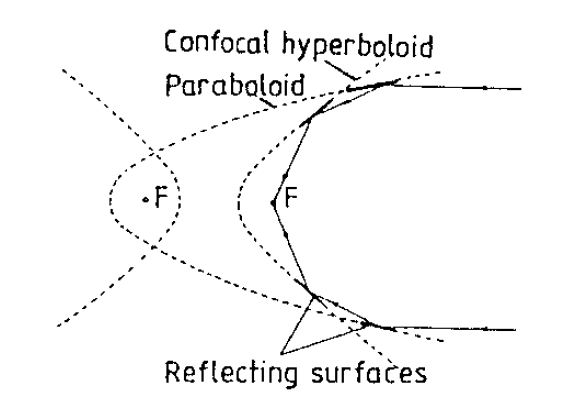
\includegraphics[width=.4\textwidth]{Immagini/Chapter2/Wolter1}}
%
\subfloat[][Wolter II \label{fig: Wolter2}]
   {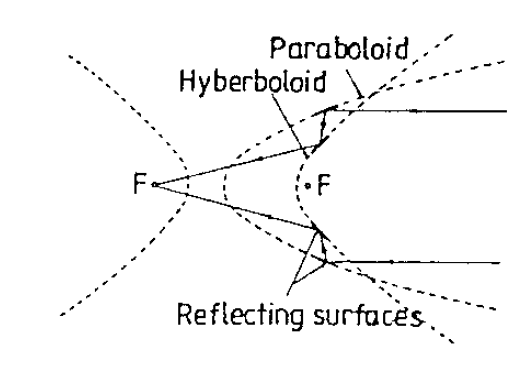
\includegraphics[width=.4\textwidth]{Immagini/Chapter2/Wolter2}}\quad
%
\subfloat[][Wolter III  \label{fig: Wolter3}]
   {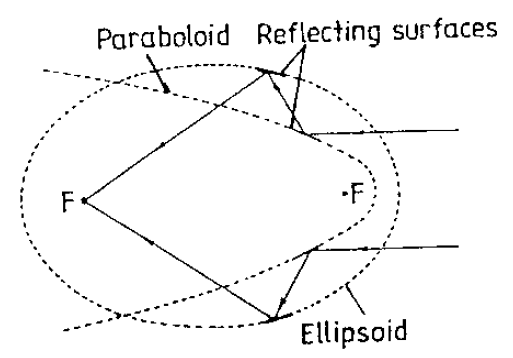
\includegraphics[width=.4\textwidth]{Immagini/Chapter2/Wolter3}}
%
\label{fig :Wolter Systems}
%
\end{figure}

\subsection{Kirkpatrick-Baez System}

\hspace{10mm} This kind of optics are used in the ESRF and consist, as shown in Figure, in two separated cylindrical surface conical mirror that focus the incident beam in both saggital and transverse thus astigmatism is removed. Although such system introduce another type of distortion, anamorphotism. Because of the different distance of the image plane with respect to the mirrors the magnification is different in the two direction.  Another technical problem that face with system is the big volume that occurs to implement it.
\noindent To overcome those two problem and obtain a system that conjugate the good behaviour of the KB system with an equal magnification of the two direction and compact system, it is possible to implement a system as it is showed in Figure, a system in which both mirrors are at the same distance from the object. This sort of arrangement is extremely difficult to manufacture and, consequently, very expensive.
\noindent Despite these problem K-B system are very used in ESRF and in European synchrotron, on the contrary, in American synchrotron another type of optical system, named "Montel", is used that will be discussed in the next section.
\begin{figure}[H]
%
\centering
%
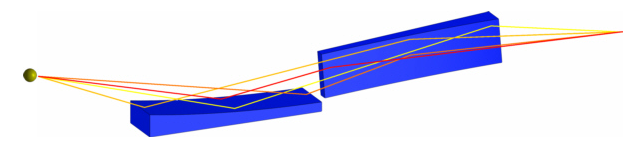
\includegraphics[width=.6\textwidth]{Immagini/Chapter2/KBSystem}
%
\caption{Kirkpatrick-Baez system}
%
\label{fig: SurfaceConic1}
%
\end{figure}


\section{Montel}

\hspace{10mm} As discussed before KB system have some limitation that can be overcome with a different optical system named "Montel". This geometry bring four important advantages for high-precision focusing: 
\\ i) the optical system is more compact which allow greater working space;
\\ ii) the focal distance of the two mirror are the same, this cancel out  the anamorphotism;
\\ iii) the alineation of the system is easier with respect to the KB system because, in this case, only one thing has to be aligned, however , in the KB there are two separated mirror that has to be aligned;
\\ iv) the divergence that can be collected is larger which allows for greater flux and/or a lower diffraction limit.
\begin{figure}[H]
%
\centering
%
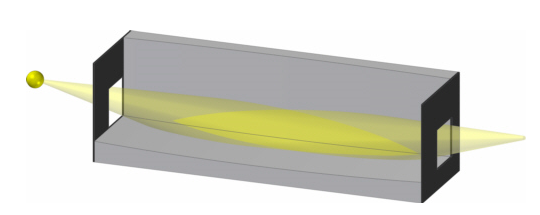
\includegraphics[width=.6\textwidth]{Immagini/Chapter2/MontelSystem}
%
\caption{Montel system}
%
\label{fig: SurfaceConic1}
%
\end{figure}

\subsection{Diffraction limit of Montel compared to sequential K:}
The image quality and dimension, for x-rays reflective optics, is  caused by aberration, mirror imperfection, and magnification of the system. Nowadays it is possible to create a mirror with high surface quality with a so high demagnification that the spot focal size is limited,p primary, by diffraction and mechanical/environmental factors.
\begin{figure}[H]
%
\centering
%
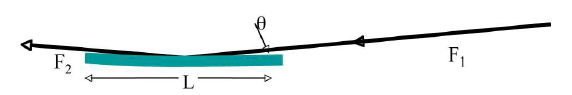
\includegraphics[width=.7\textwidth]{Immagini/Chapter2/System3}
%
\caption{Standard parameters that define an elliptical mirror}
%
\label{fig: System3}
%
\end{figure}
The first limiting factor (diffraction) depends on the wavelengths of the radiation and on the divergence of the Beam. Figure \ref{fig: System3} show a simple elliptical mirror with an object focal of $F_1 $, an image focal of $F_2 $, an incidence angle $\theta $ and a length of the mirror equal to $L $. For piraticpraticalal calculation it is convenient to use the system in Figure \ref{fig: System4} , where $F_d $ is the distance from the end of the mirror to the image focal, $\theta_i $ the divergence focused at the image point, $\theta_d $ the maximum accepted angle, $\theta_o $, the divergence intercepted by the mirror.
\\
For an elliptical KB system the FWHM of the diffraction limit in each plane is:
\begin{equation}
D_{FWHM} \sim  \frac{0.88 \lambda}{\theta_i}
\label{eq: D_FWHM}
\end{equation}
\noindent where $\lambda $ is the wavelength of the radiation. For the total external reflection that rules the reflection for the X-ray, the maximum divergence that can be collected is that which correspond to the critical angle $\theta_c $, that can be calculated as
\begin{equation}
\theta_c \sim \sqrt{\rho \delta} = 6.7 10^{-2} \lambda (nm) = \frac{8.4 10^{-2}}{E(keV)}
\label{eq: theta_c}
\end{equation}
\noindent In reality, due to geometrical constrain on sequential KB system, the maximum divergence that can be collected is about $0.84 \theta_c $.
\begin{figure}[H]
%
\centering
%
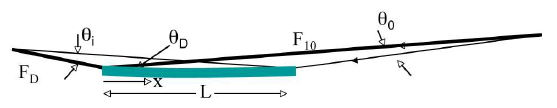
\includegraphics[width=.7\textwidth]{Immagini/Chapter2/System4}
%
\caption{New parameter that define an elliptical mirror, useful for calculation}
%
\label{fig: System4}
%
\end{figure}
%
To study the diffraction limit of a KB system, it is done a theorical treatment of micro focusing using elliptical mirror, and working on the parameter that define the geometrical shape, using the system in Figure \ref{fig: System4}. The image and objective divergence, $\theta_i $ and $\theta_o $, depend on the angle $\theta_d $, the ratio $L $ over $F_d $, length of the mirror over the distance between the image focus and the end of the mirror, and the angle $\theta_d $.
%
\begin{figure}[]
%
\centering
%
\subfloat[][Plot2 \label{fig: Plot1a}]
   {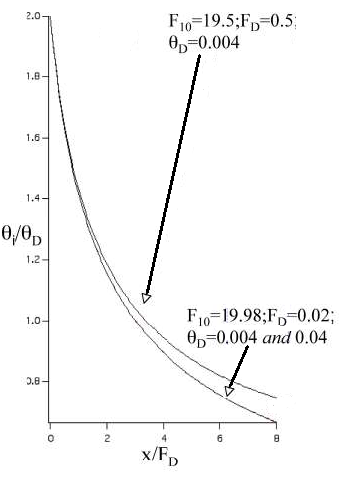
\includegraphics[width=.5\textwidth]{Immagini/Chapter2/Plott1}}
%
\subfloat[][Plot3  \label{fig: Plot1b}]
   {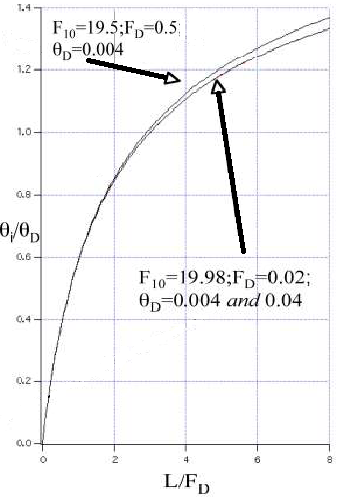
\includegraphics[width=.5\textwidth]{Immagini/Chapter2/Plott2}} \quad
%
\subfloat[][Plot3  \label{fig: Plot1c}]
   {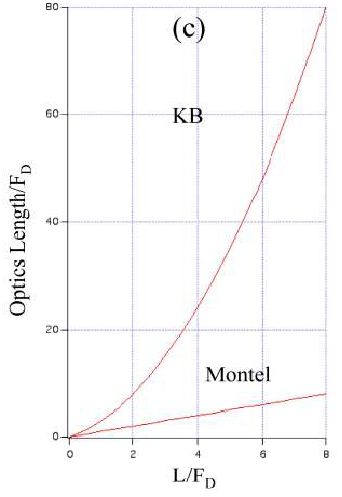
\includegraphics[width=.5\textwidth]{Immagini/Chapter2/Plott3}}
%
\caption{Plots}
\label{fig: Plot1}
%
\end{figure}
%
\noindent Figure \ref{fig: Plot1a} can be used to estimate the fraction of the mirror that can reflect different wavelengths. If the mirrpr is designed to work for the wavelength $\lambda $ with $\theta_d = \theta_c $, a new wave with wavelength equal to $\lambda / 2 $, the part of the mirror that is covered is that with $x / F_d > 3.5$ reflect efficiently the radiation. With Figure \ref{fig: Plot1b}  it is possible to estimate the radiation collect at the image plane. Normalizing the length of the mirror with $F_d $ and, normalizing the divergence angle collected with the biggest angle $\theta_d $, then the normalized numbers fall down to a universal curve aass menobhysa di a foactor of 10-20. This curve is useful because it can estimate the radiation collected by the KB/Montel.For example, if $L/F_d $ is n for each mirror of the KB system, then the total length of the system is related to the clearance distance of the second mirror
\begin{equation}
L= (2 n + n^2 ) F_d
\label{eq: clearance distance}
\end{equation}
\noindent for the Montel system the total length is only $L = n F_d $. In Figure \ref{fig: Plot1c} is showed the length of both compound system, and, for large  $n>2 $ the situation is dramatical, for example for $n=2 $ KB length is about the same of Montel with $n=8 $. This mean that the diffraction limit for total external reflection for KB is about $16 nm$, for Montel $11 nm$.
\\
Mirrors can be designed to work well with short or medium or large wavelengths. Depending on the design, the diffraction  limit is limited to certain conditions. If the mirrors are designed for short wavelength, according to Equation \ref{eq: D_FWHM}, the diffraction limit is mainly governed by the wavelength, because the divergence collected is roughly independent from the wavelength. On the contrary, if the mirror are optimized to long wavelengths, the surface that reflect the radiation is only a fraction, this compromise the shortest wavelength. Figure \ref{fig: Plot2} show the dependace of the diffraction limit with mirror designed to be optimize, with the choice of the $\theta_d $ to different situation.
%
%
\begin{figure}[]
%
\centering
%
\subfloat[][Plot2 \label{fig: Plot2}]
   {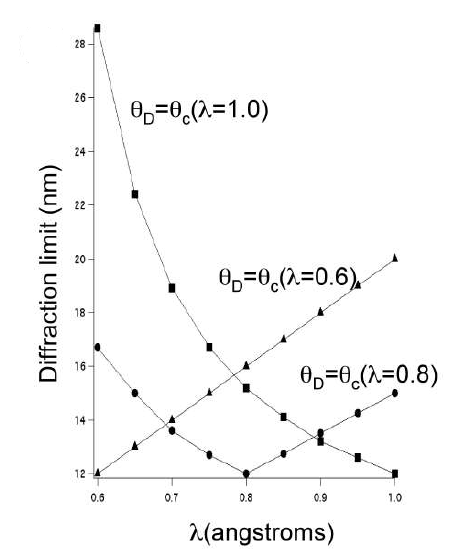
\includegraphics[width=.5\textwidth]{Immagini/Chapter2/Plot2}}
%
\subfloat[][Plot3  \label{fig: Plot3}]
   {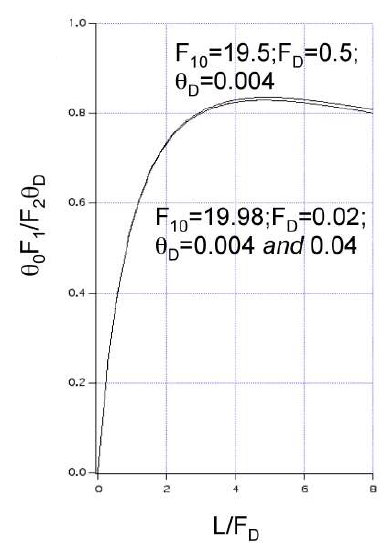
\includegraphics[width=.5\textwidth]{Immagini/Chapter2/Plot3}}
%
\caption{Plots}
\label{fig: Plot1}
%
\end{figure}
%
\subsection{Flux limit}
If the beam is small, the flux is the limitating factor to the image spot. For the KB optics designed to demagnify the source, increasing the length of the mirror than the collected divergence increase, the backdraw is that the demagnification decrease, in the sense that became less strong, so, to reobtaine the desired image dimension it have to decrease the object spot. The geometrical demagnification is, according to Figure \ref{fig: System4},
\begin{equation}
\frac{F_d (1 + n / 2 )}{F_10 - n F_d / 2} =\frac{F_2}{F_1}
\label{eq: geometrical demag}
\end{equation}
\noindent and the collect divergence of the radiation at the image plane is $\theta_0 $. As it is reported in Figure \ref{fig: Plot3}, the performance fall down to another universal curve for large and small demagnification.
\\
In this case the Montel system is better than the KB optics because of the largeer numerical aperture that increase the flux on the sample. This last point is convenient for neutron experimental uses where the flux limit overcame the diffraction limit, differently than the X-ray experiments. Montel flux is 2.6 times increase with respect to the KB. A Montel long $0.25m $ of clearance has $n = 2 $, a similar value to the longest of the mirror give an $n \sim 0.73 $, with a difference in the total flux collect into a small spot of $\sim 2.5$.
\subsection{Optical Design}

The mirrors used in this Montel configuration are mirror that have a cylindrical shape in one direction and elliptical shape in the other direction. One approach to obtain the Montel system is that to use two pre-figured elliptical mirror and grind the cut site at 45$^\circ $ as shown in figure. After that it place the mirrors together makes a good fit with no gap requiring no contouring of the mirror side. Another way involves diveding pre-figured elliptical mirror into two part that, add them together, can form the Montel system. This approaches is primary driven by the fact that in a conventionally polished mirror, the clear aperture area has the best figure and finish. As such uAs such, using two halves of a prefigured mirror cut in the middle has several advantages- including consistency and economy. There are major challenges
however. First, the mirror surface must be protected against damage and deformation during cutting and subsequent figuring operations. After cutting into two, the cut sites must be treated (e.g., etched) to remove any subsurface damages that could alter a mirror's figure. Then the mating side of one of the mirrors must be contoured and polished such that when it is placed against the partner mirror, it makes a nearly perfect fit with good surface quality all the way to the contact edge.This last two-steps are crucial because if there is a significant gap or if the mirror surfaces in the vicinity of the interface are damaged, a significant part of the incident beam could be lost. As an example, we are developing a pair of Montel mirrors for polychromatic nanofocusing on Sector 33 at APS. This beam line will use 40 mm long elliptical mirrors for nano-focusing a 100 $\mu m$ beam to a 50 nm spot at 2000x demagnification. This concave elliptical mirror has a maximum depression of about 6 $\mu m$ at its center. If cut flat and placed against its mating mirror, a gap as large as 6 $\mu m$ is created which loses about 10$\% $ of the 100 $\mu m$ incident beam. Similarly, if the mirror surfaces near the intersection are damaged, then beam loss can be significant.
\begin{figure}[]
%
\centering
%
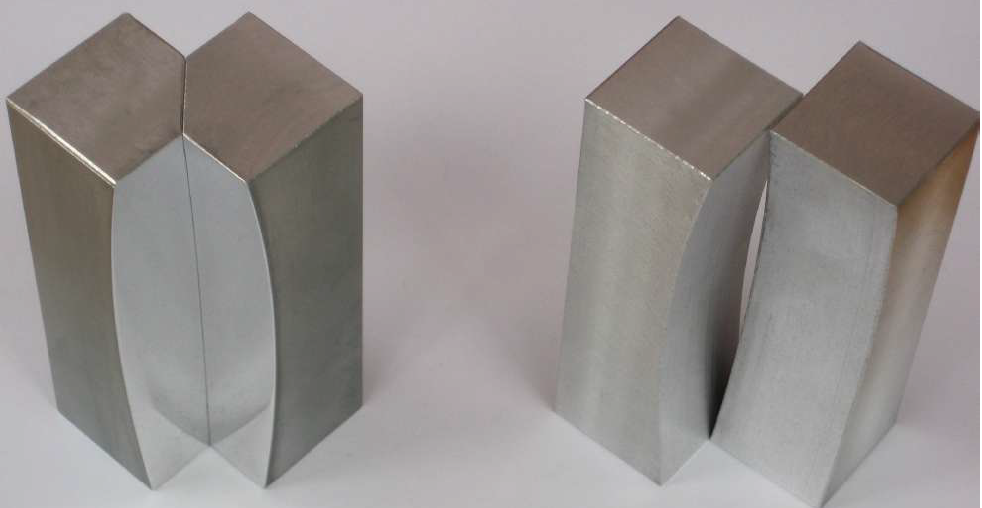
\includegraphics[width=.8\textwidth]{Immagini/Chapter2/MontelEdges}
%
\caption{Example in how to build a Montel system starting from two cilindrical mirror cutting the edge with ad angle of $45^{\circ} $.}
%
\label{fig: MontelEdges}
%
\end{figure}

%
%\chapter{Montel System}
\label{capitolo3}
\thispagestyle{empty}

\vspace{0.5cm}

\section{Montel}

\hspace{10mm} As discussed before KB system have some limitation that can be overcome with a different optical system named "Montel". This geometry bring four important advantages for high-precision focusing: 
\\ i) the optical system is more compact which allow greater working space;
\\ ii) the focal distance of the two mirror are the same, this cancel out  the anamorphotism;
\\ iii) the alineation of the system is easier with respect to the KB system because, in this case, only one thing has to be aligned, on the contrary, in the KB there are two separated mirror that has to be aligned;
\\ iv) the divergence that can be collected is larger which allows for greater flux and/or a lower diffraction limit.

\subsection{Optical Design}

The mirrors used in this Montel configuration are mirror that have a cylindrical shape in one direction and elliptical shape in the other direction. One approach to obtain the Montel system is that to use two pre-figured elliptical mirror and grind the cut site at 45$^\circ $ as shown in figure. After that it place the mirrors together makes a good fit with no gap requiring no contouring of the mirror side. Another way involves diveding pre-figured elliptical mirror into two part that, add them together, can form the Montel system. This approaches is primary driven by the fact that in a conventionally polished mirror, the clear aperture area has the best figure and finish. As such uAs such, using two halves of a prefigured mirror cut in the middle has several advantages- including consistency and economy. There are major challenges
however. First, the mirror surface must be protected against damage and deformation during cutting and subsequent figuring operations. After cutting into two, the cut sites must be treated (e.g., etched) to remove any subsurface damages that could alter a mirror's figure. Then the mating side of one of the mirrors must be contoured and polished such that when it is placed against the partner mirror, it makes a nearly perfect fit with good surface quality all the way to the contact edge.This last two-steps are crucial because if there is a significant gap or if the mirror surfaces in the vicinity of the interface are damaged, a significant part of the incident beam could be lost. As an example, we are developing a pair of Montel mirrors for polychromatic nanofocusing on Sector 33 at APS. This beam line will use 40 mm long elliptical mirrors for nano-focusing a 100 $\mu m$ beam to a 50 nm spot at 2000x demagnification. This concave elliptical mirror has a maximum depression of about 6 $\mu m$ at its center. If cut flat and placed against its mating mirror, a gap as large as 6 $\mu m$ is created which loses about 10$\% $ of the 100 $\mu m$ incident beam. Similarly, if the mirror surfaces near the intersection are damaged, then beam loss can be significant.
%
\chapter{Montel System}
\label{capitolo3}
\thispagestyle{empty}

\vspace{0.5cm}

\section{Montel}

\hspace{10mm} As discussed before KB system have some limitation that can be overcome with a different optical system named "Montel". This geometry bring four important advantages for high-precision focusing: 
\\ i) the optical system is more compact which allow greater working space;
\\ ii) the focal distance of the two mirror are the same, this cancel out  the anamorphotism;
\\ iii) the alineation of the system is easier with respect to the KB system because, in this case, only one thing has to be aligned, on the contrary, in the KB there are two separated mirror that has to be aligned;
\\ iv) the divergence that can be collected is larger which allows for greater flux and/or a lower diffraction limit.

\subsection{Optical Design}

The mirrors used in this Montel configuration are mirror that have a cylindrical shape in one direction and elliptical shape in the other direction. One approach to obtain the Montel system is that to use two pre-figured elliptical mirror and grind the cut site at 45$^\circ $ as shown in figure. After that it place the mirrors together makes a good fit with no gap requiring no contouring of the mirror side. Another way involves diveding pre-figured elliptical mirror into two part that, add them together, can form the Montel system. This approaches is primary driven by the fact that in a conventionally polished mirror, the clear aperture area has the best figure and finish. As such uAs such, using two halves of a prefigured mirror cut in the middle has several advantages- including consistency and economy. There are major challenges
however. First, the mirror surface must be protected against damage and deformation during cutting and subsequent figuring operations. After cutting into two, the cut sites must be treated (e.g., etched) to remove any subsurface damages that could alter a mirror's figure. Then the mating side of one of the mirrors must be contoured and polished such that when it is placed against the partner mirror, it makes a nearly perfect fit with good surface quality all the way to the contact edge.This last two-steps are crucial because if there is a significant gap or if the mirror surfaces in the vicinity of the interface are damaged, a significant part of the incident beam could be lost. As an example, we are developing a pair of Montel mirrors for polychromatic nanofocusing on Sector 33 at APS. This beam line will use 40 mm long elliptical mirrors for nano-focusing a 100 $\mu m$ beam to a 50 nm spot at 2000x demagnification. This concave elliptical mirror has a maximum depression of about 6 $\mu m$ at its center. If cut flat and placed against its mating mirror, a gap as large as 6 $\mu m$ is created which loses about 10$\% $ of the 100 $\mu m$ incident beam. Similarly, if the mirror surfaces near the intersection are damaged, then beam loss can be significant.
%
\chapter{Test and Results}
\label{capitolo4}

\vspace{5cm}

In the first part of the Chapter is tested the correct working of the MONWES library. The test for mirrors, ideal lens and KB is done against OASYS software. For the Montel system, because it is not implemented in OASYS, it is done a benchmark with the paper \cite{resta2015nested}.
\\
The second part of the Chapter use the MONWES library to study the behaviour of the Montel system. It is studied the effect of a non-centred beam watching what happen to the image dimension and the intensity in the case of centred and non centred beam. At the end it is reported the study that I have done, for the beamline ID20 of the ESRF, of a non-orthogonal Montel mirrors.
\vspace{0.5cm}
\section{Testing against OASYS}
%
OASYS (OrAnge SYnchrotron Suite) is a graphical environment for optic simulation used in synchrotron facilities based on orange 3, developped by Manuel Sanchez Del Rio (ESRF) and Luca Rebuffi (ELETTRA).
The comparison between the program and the OASYS software is done with the system in Figure \ref{fig: Optical system}. In this system the 1st optical system collimate the source and the 2nd optical system focalize the Beam at the image plane. The different lentgth that characterize the system are: between the source and the 1st optical system there is a  distance of  $d_1 = f = 0.4 m $, between the 2st and the 2nd optical system a distance $d_2 = 0.6 m $ and the distance between the 2nd system and the image plane correspond to a distance of $d_3 = f = 0.4$. A system that have parameters defined as before, make a copy of the source image at the image plane.
%
\begin{figure}[]
%
\centering
%
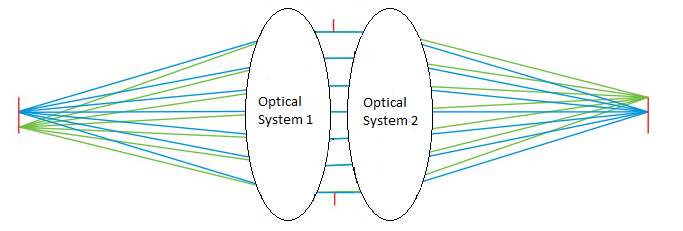
\includegraphics[width=.6\textwidth]{Immagini/Chapter4/OpticalSystems}
%
\caption{Optical system used for the test with OASYS}
%
\label{fig: Optical system}
%
\end{figure}
%
The source parameter used are showed in Figure \ref{fig: Source Parameter for OASYS}, and correspond to  a square source spot of $1 \mu m^2 $, and a initial Gaussian divergence with a FWHM of $2.3 mrad $.
\begin{figure}[]
%
\centering
%
\subfloat[][Initial spot size \label{fig: Source OASYS}]
   {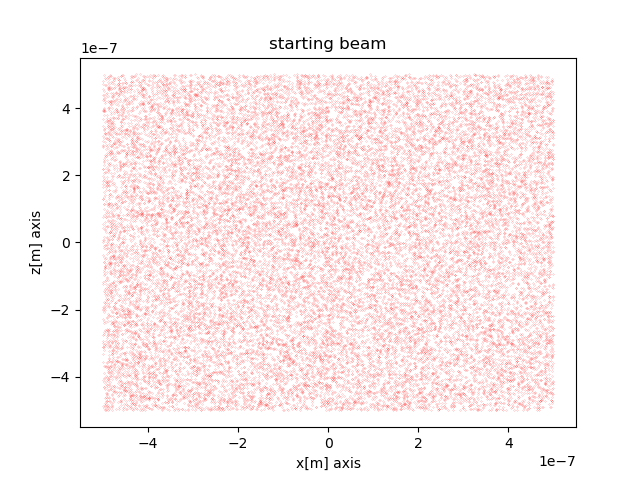
\includegraphics[width=.4\textwidth]{Immagini/Chapter4/SouceOASYS}}
%
\subfloat[][Initial Beam divergence\label{fig: Divergence OASYS}]
   {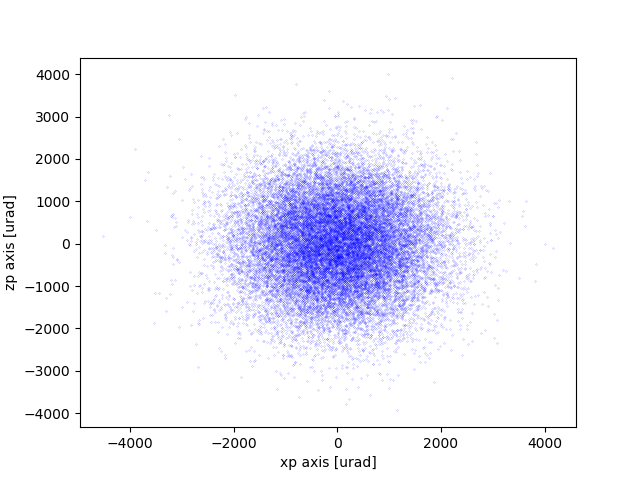
\includegraphics[width=.48\textwidth]{Immagini/Chapter4/DivergenceOASYS}}
%
\caption{Parameter of the source used for the test with OASYS}
%
\label{fig: Source Parameter for OASYS}
%
\end{figure}
%
The tests is done using different optical system, with the same focal length and, for the mirror, with a grazing incidence angle of $\theta = 1.719^{\circ}$. Below are plotted the image of the Beam at the image plane, putting the OASYS results on the right, and my results on the left. 
\\
The system simulated are done with:
\begin{enumerate}
\item ideal lenses Figure \ref{fig: Ideal lense OASYS}
\item parabolic mirror Figure \ref{fig: paraboloid OASYS}
\item KB system Figure \ref{fig: KB system OASYS}
\end{enumerate} 
\noindent As it is showed in the figures \ref{fig: Ideal lense OASYS}, \ref{fig: paraboloid OASYS} and KB system Figure \ref{fig: KB system OASYS}, the result, of OASYS and my simulations are in good agreement. The ideal lenses case show a perfect replica of the source image, on the contrary, KB and paraboloid, show similar images but a bit aberrated, because it degrades along the propagation.
\newpage
%
\begin{figure}[H]
%
\centering
%
\subfloat[][My ideal lenses simulation \label{fig: my Ideal Lenses}]
   {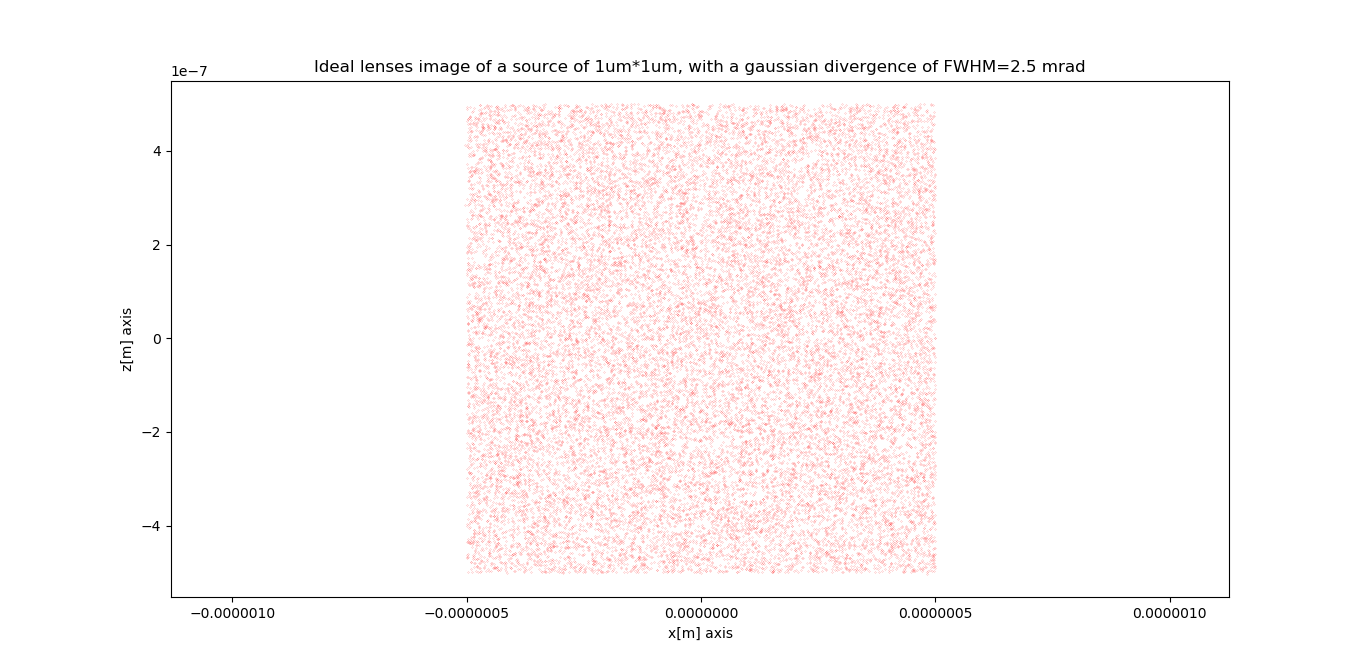
\includegraphics[width=.5\textwidth]{Immagini/Chapter4/IdealLens}}
%
\subfloat[][OASYS ideal lenses simulation \label{fig: Ideal Lenses OASYS}]
   {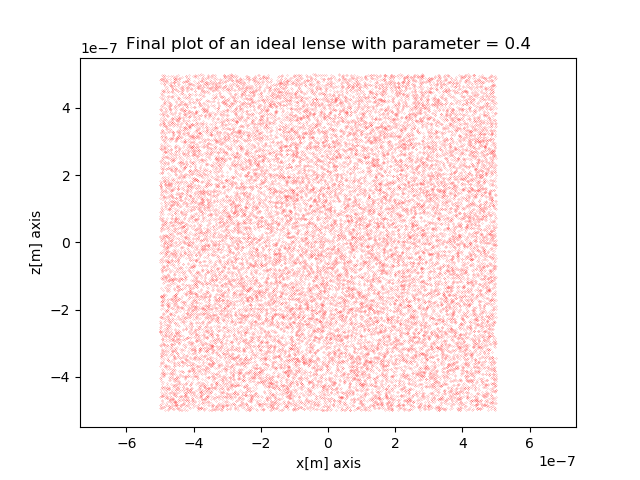
\includegraphics[width=.5\textwidth]{Immagini/Chapter4/IdealLensOASYS}}
%
\caption{Image for the testing ideal lenses system in Figure \ref{fig: Optical system} of: my simulation (Figure \ref{fig: my Ideal Lenses}) and OASYS simulation (Figure \ref{fig: Ideal Lenses OASYS})}
%
\label{fig: Ideal lense OASYS}
%
\end{figure}
%
\begin{figure}[H]
%
\centering
%
\subfloat[][My paraboloid simulation \label{fig: my Paraboloid}]
   {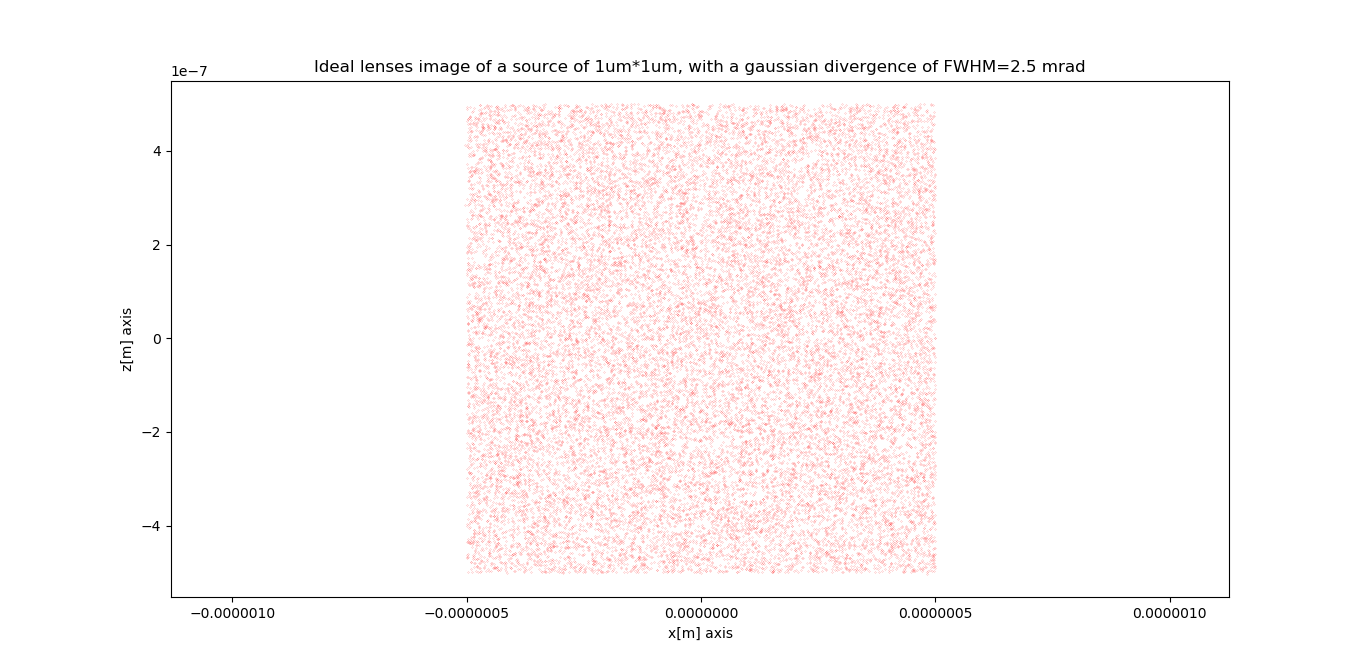
\includegraphics[width=.5\textwidth]{Immagini/Chapter4/IdealLens}}
%
\subfloat[][OASYS paraboloid simulation \label{fig: Paraboloid OASYS}]
   {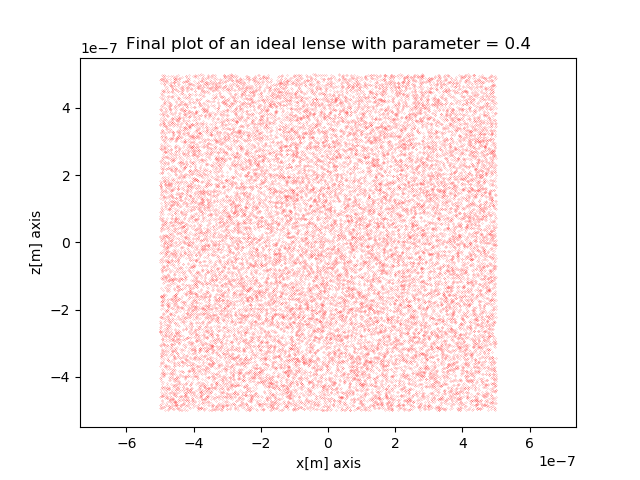
\includegraphics[width=.5\textwidth]{Immagini/Chapter4/IdealLensOASYS}}
%
\caption{Image for the testing paraboloid system in Figure \ref{fig: Optical system} of: my simulation (Figure \ref{fig: my Paraboloid}) and OASYS simulation (Figure \ref{fig: Paraboloid OASYS})}
%
\label{fig: paraboloid OASYS}
%
\end{figure}
%
\begin{figure}[H]
%
\subfloat[][My KB simulation \label{fig: my KB}]
   {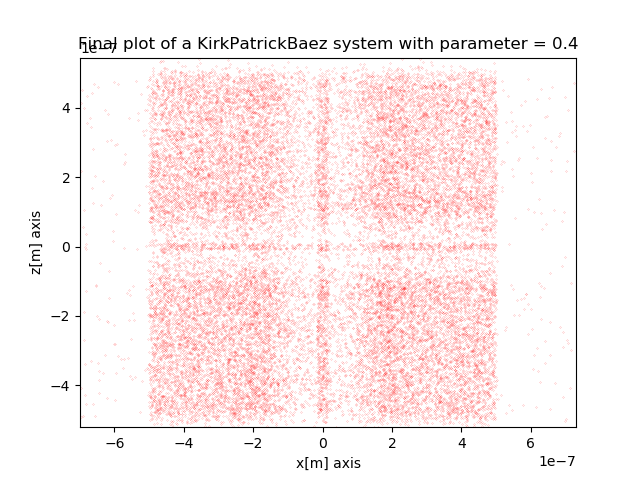
\includegraphics[width=.5\textwidth]{Immagini/Chapter4/KB}}
%
\subfloat[][OASYS KB divergence\label{fig: KB OASYS}]
   {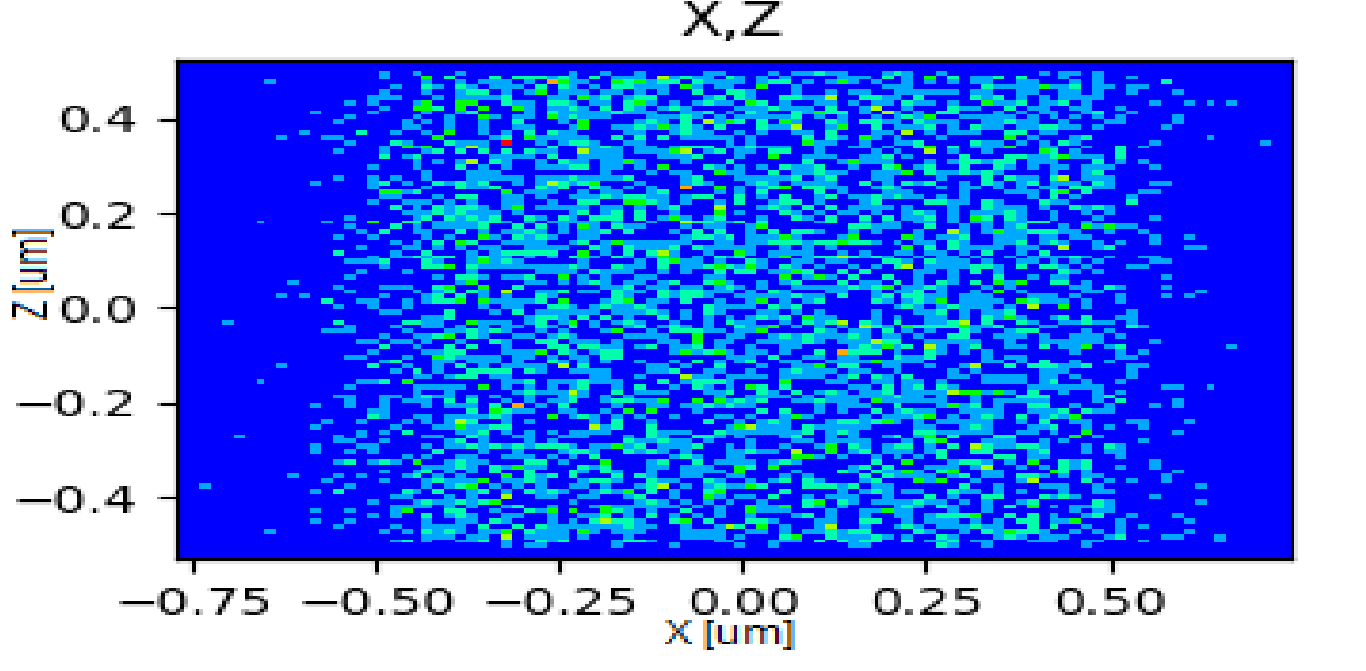
\includegraphics[width=.5\textwidth]{Immagini/Chapter4/KBOASYS}}
%
\caption{Image for the testing KB system in Figure \ref{fig: Optical system} of: my simulation (Figure \ref{fig: my KB}) and OASYS simulation (Figure \ref{fig: KB OASYS})}
%
\label{fig: KB system OASYS}
%
\end{figure}
%
\newpage
%
\subsection{Benchmarking} 
The system used for the benchmarking is showed in Figure \ref{fig: PaperMontelSystem} using the reference frame of the paper \cite{resta2015nested}. The aim of this system is to collimate a Beam using a Montel with two parabolic mirrors. The source used has a Gaussian dimension of 2.5$\mu $m FWHM and a Gaussian divergence of 5$mrad $. The distances, between the source/image plane and the center of the Montel are, respectively,  $\simeq $ 0.26m and 10.06m. The incidence angle of the Beam is $\theta_g \simeq 2.86^{\circ} $.
%
\begin{figure}[]
	\centering
		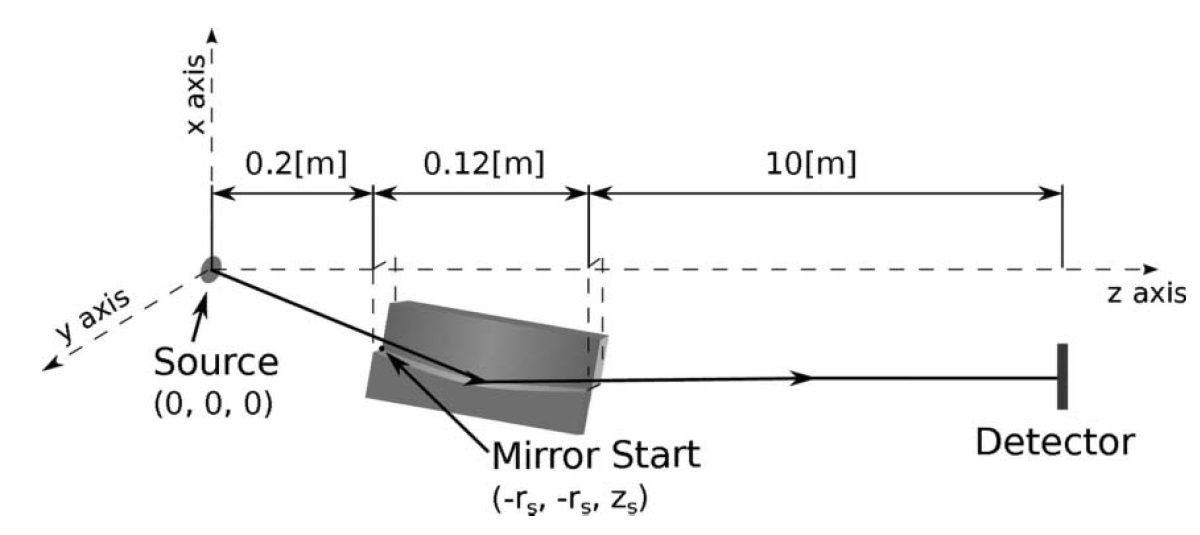
\includegraphics[width=0.8\textwidth]{Immagini/Chapter4/PaperMontelSystem}
		\caption{Illustration of the Montel system used as a collimator in the paper \cite{resta2015nested}}
		\label{fig: PaperMontelSystem}
\end{figure}
%
The result, at the image plane, of the beam size and beam divergence, after the double-reflection of the Montel system, is showed in Figure \ref{fig: My Simulation Comparison}. There in Figure \ref{fig: PaperImageShape} shows the beam at the image plane, and  Figure \ref{fig: PaperImageDivergence}shows the divergence. The quantitative values reported on the paper correspond to a Gaussian-like distribution with a spatial FWHM of $\sim $0.7mm for the spot size, and a FWHM of the Gaussian divergence $\sim $ 0.01 mrad.
\\
Repeating the simulation with MONWES, and using the parameter defined in  in the paper \cite{resta2015nested} it obtain Figure \ref{fig: My Simulation Comparison}. As it is showed in the Figure \ref{fig: My Simulation Comparison} there are a qualitative good agreement between the two simulation. Also, under a quantitative point of view, there is a good agreement in fact, in my simulation are obtained a value of $\sim $1mm of FWHM of image size, pretty similar to the one of the other simulation, and $\sim $0.01 mrad FWHM of divergence that is equal to the one obtained with the other simulation.
%
\begin{figure}[]
%
\centering
%
\subfloat[][Beam image shape of the paper\label{fig: PaperImageShape}]
   {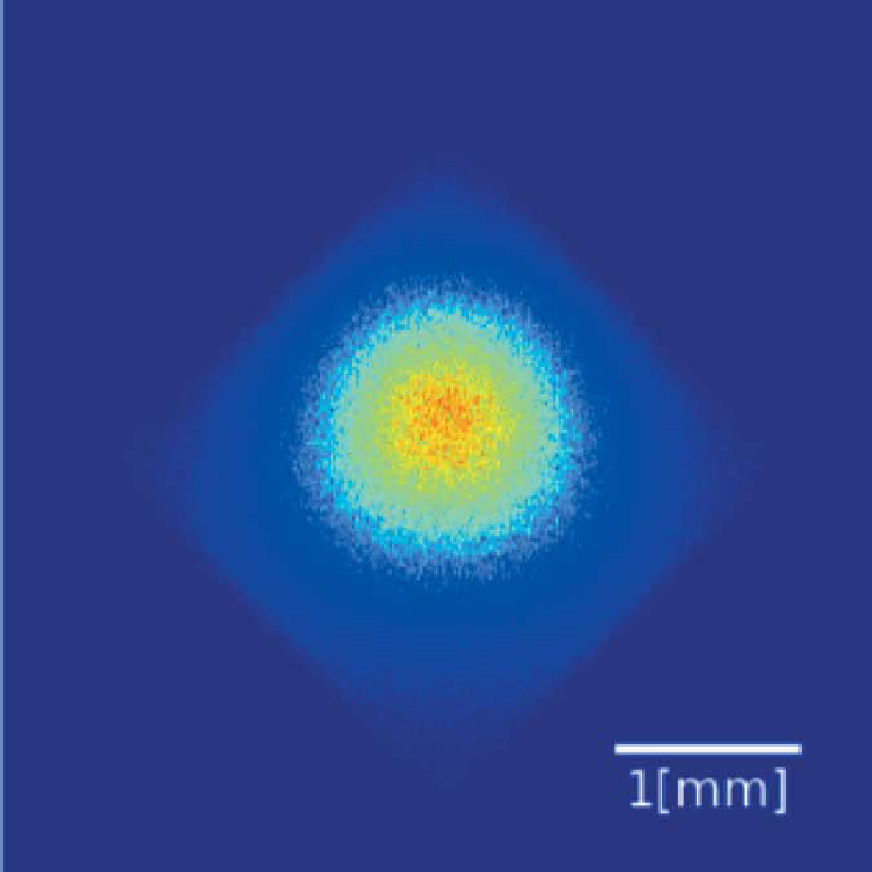
\includegraphics[width=.4\textwidth]{Immagini/Chapter4/PaperSpotMontel}}
%
\subfloat[][Beam image shape of the simulation\label{fig: Image dimension}]
   {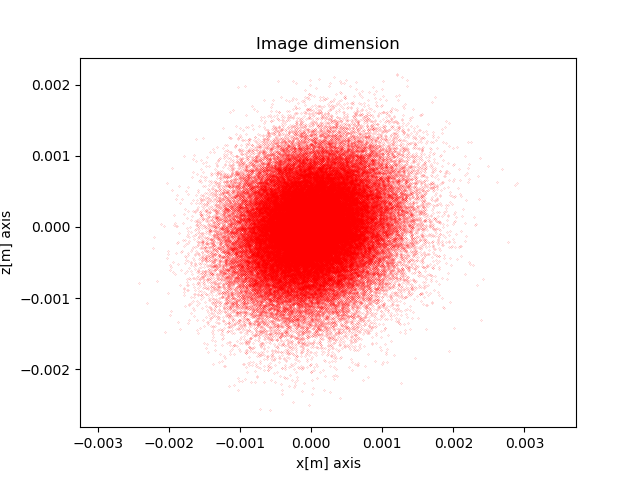
\includegraphics[width=.48\textwidth]{Immagini/Chapter4/ImageDimension}}\quad
%
\subfloat[][Beam image divergence of the paper\label{fig: PaperImageDivergence}]
   {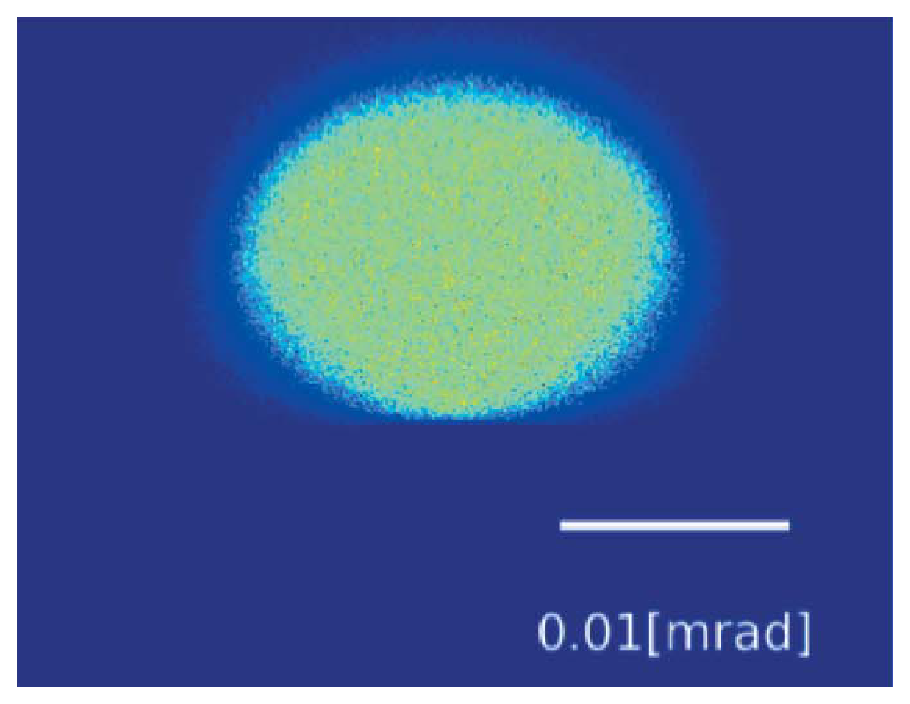
\includegraphics[width=.4\textwidth]{Immagini/Chapter4/PaperDivergenceMontel}}
%
\subfloat[][Beam image divergence of the simulation\label{fig: Divergence dimension}]
   {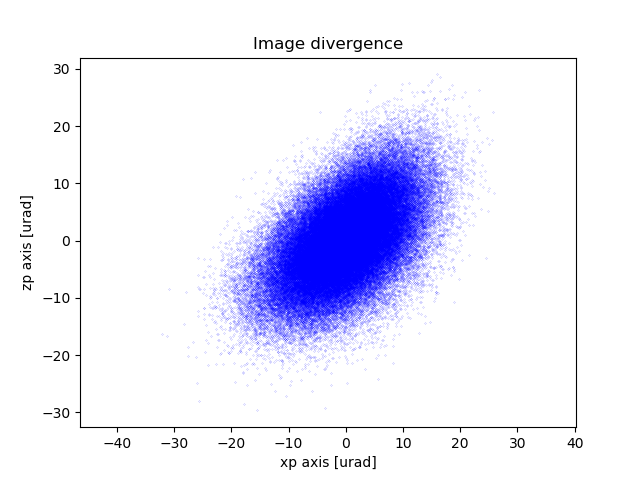
\includegraphics[width=.48\textwidth]{Immagini/Chapter4/DivergenceDimension}}
%
\caption{Results of  the Montel simulations with a source beam with a FWHM spot of 2.5$\mu $m and a Gaussian divergence of 5$mrad $}
%
\label{fig: My Simulation Comparison}
%
\end{figure}
%
\section{Analysis of Montel system}
In this section a study of the Montel is done, using the Montel tools developed. The first simulation, to verify that Montel work well, study the behaviour of a point-wise source with a certain divergence, using a collimating system. The second simulation, for the same reason of before, simulates a collimating beam with a certain source shape geometry and figure out the image plot obtained by a focalizing system in its image plane. What is expected is a point in the divergence space for the first situation and in the real space for the second simulation, as a consequence of the ideal collimating/focalizing system. For the simulation parabolic Montel with an incidence angle of 2$^{\circ} $ (the choice of the angle is arbitrary) are used. Paraboic system are chosen because is the only way to obtain a perfect collimating Beam.
\\
Figure \ref{fig: ideal} reports the result for the ideal collimating/focalizing cases.
For the collimation system a point wise source  is used with a Gaussian divergence of FWHM of 25$\mu $m, \ref{fig: coll.Source}. At the image plane the Beam (Figure \ref{fig: CollimationImage}) is collimated, reducing its divergence of 3 orders of magnitude. For the focalizing system, it is used a circular source spot having a radius of 1mm, Figure \ref{fig: foc.Source}, with a collimated source beam. At the image plane the dimension of the Beam (Figure \ref{fig: focalizingImage}) is reduced of 3 order magnitude. It is possible to conclude that both collimating and focalizing system work but not perfectly (the final results are not point). One explanation can be that, because of the particular configuration of the mirrors of the Montel, the effect on the Beam are not perfect. This can be an \textbf{intrinsic aberration of the Montel}, that can be studied more in the future.
\\
\begin{figure}[]
%
\centering
%
\subfloat[][Source divergence\label{fig: coll.Source}]
   {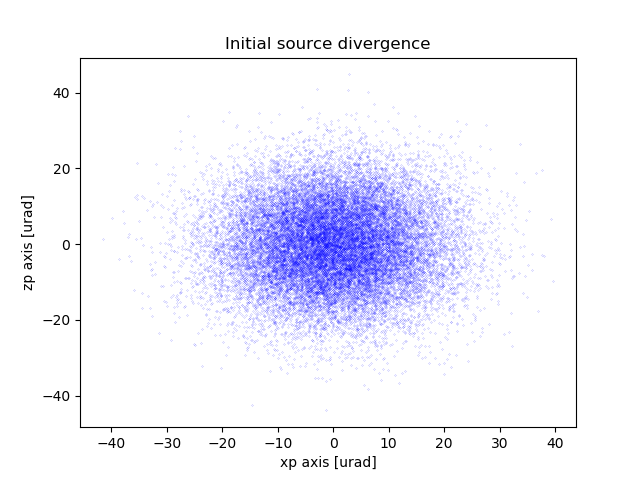
\includegraphics[width=.4\textwidth]{Immagini/Chapter4/CollimationSource}}
%
\subfloat[][Image divergence\label{fig: CollimationImage}]
   {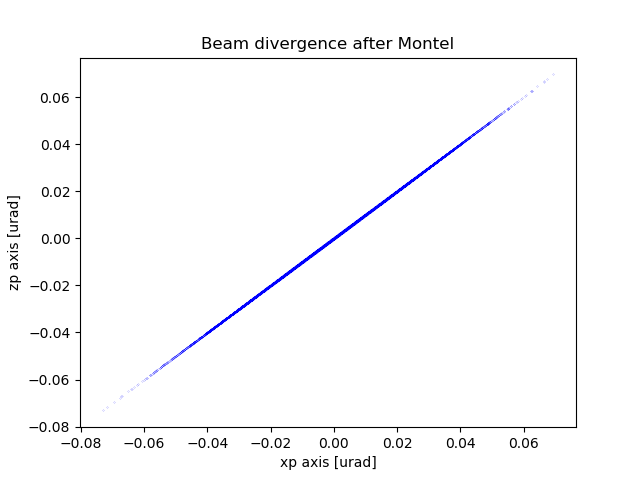
\includegraphics[width=.4\textwidth]{Immagini/Chapter4/CollimationImage}}\quad
%
\subfloat[][Source divergence\label{fig: foc.Source}]
   {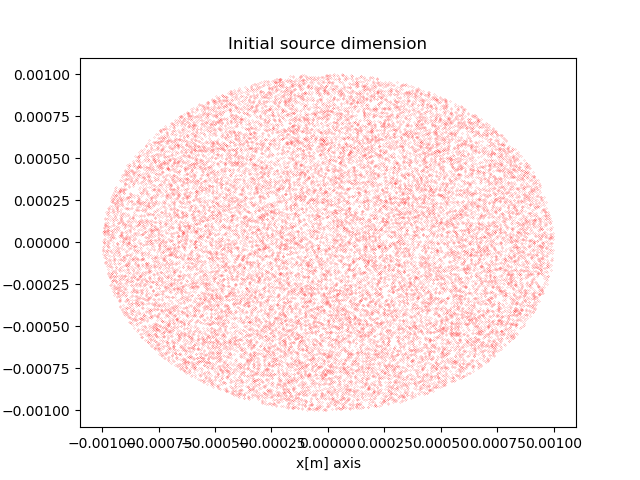
\includegraphics[width=.4\textwidth]{Immagini/Chapter4/FocalizingSource}}
%
\subfloat[][Image divergence\label{fig: focalizingImage}]
   {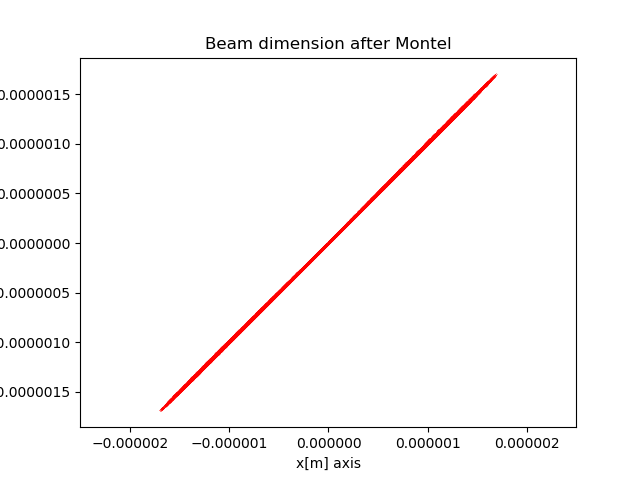
\includegraphics[width=.4\textwidth]{Immagini/Chapter4/FocalizingImage}}
%
\caption{Ideal system}
%
\label{fig: ideal}
%
\end{figure}
%
Up to now the dimension of the Montel were not considered. The Montel is set to have infinite dimension in all the direction. This approach hold in the case of a small source and a narrow profile divergence, that hit only a small part of the system. Otherwise, for example of an isotropic source that can be modelled with a very big divergence, the situation change. In this part, to study to behaviour of a big source, it is used a Beam source with a square shape with a side of 1mm, with a Gaussian profile divergence of FWHM=1mrad. These parameter show what happen to the Montel where it is covered over all its surface. I  this case a focalizing parabolic Montel is used with:  object  distance of 1m, image distance of 3m, incidence angle of $2^{\circ} $,  length of the Monte of 0.1m and width of the Montel of 20cm.
%
\begin{figure}[]
%
\centering
%
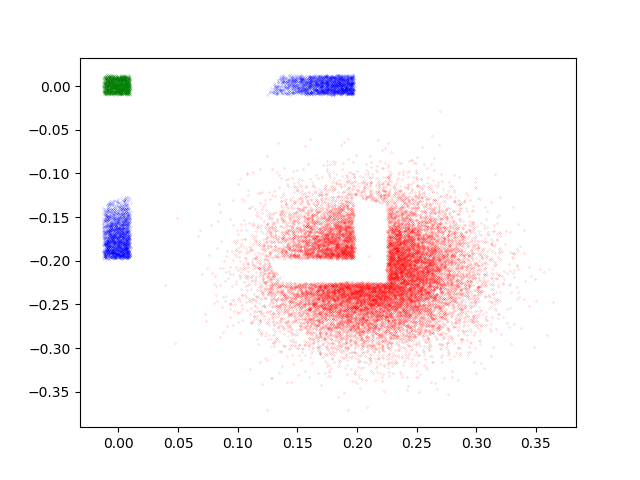
\includegraphics[width=.6\textwidth]{Immagini/Chapter4/BigSourceMontel}
%
\caption{Illumination at the image plane of the different Beam (red dots correspond to np-reflected rays, blue dot to one-reflected rays, green dots to two-reflected rays).}
%
\label{fig:BigSourceMontel}
%
\end{figure}
%
Figure \ref{fig:BigSourceMontel}, show thee image plane of the Montel defined above. This plot show 4 figure, the biggest one, represented by the red dots, correspond to the rays that reach the image plane without touch the Montel, the rays coloured in blue, are those which are subject to only one reflection that are positioned in different part of the image plane depending which mirror meet, those that hit the xy-mirror correspond to the beam elongated along z, the zy-mirror correspond to the beam elongate along x. At the end, the green dots, are the rays that do both reflection and are centred to the center of the image plane by definition of it.


\section{Non-centred Beam}
In this section is studied the effect of a Montel system of a non centred-Beam in order to understand how to align correctly beam. The alignment study is study simulating a beam tha hit different point of the Montel. Is reported the behaviour about the change of FWHM of both $x^{'} $ and $z^{'} $, of a small ($1 \mu m^2 $) source with a narrow divergence ($25 \mu rad $), following different path. Figure \ref{fig: path} show the different path followed to simulate the non-centred. Every path is labelled with a name:
\begin{enumerate}
	\item Y
	\item XZ
	\item XYZ1
	\item XZY2
\end{enumerate}

\begin{figure}[]
%
\centering
%
\includegraphics[width=1.\textwidth]{Immagini/Chapter4/Cattura2}
%
\caption{Different path for simulate the non-centred beam}
%
\label{fig: path}
%
\end{figure}

The system used is a focalizing parabolic Montel with an object focal distance of 0.2m and an image focal distance of 0.9, working on miroor designe for incidence angle of $\theta_g = 2^{\circ}$. Figure \ref{fig: reuslt diff. path} show the result the two FWHM of the beam changing the incidence point of the beam moving the different paths. This point is defined with respect to the center of the Montel system that correspond to the origin (0, 0, 0). In Figure \ref{fig: Y path}, the incidence point move along y-axis, start from the point (0, 1.5mm, 0) and arriving to the point (0, -1.5mm, 0), and show, more or less, a flat behaviour of the FWHM. Figure \ref{fig: XZ path} start from the point (0, 0, 0.15mm) and arrive to (-0.15mm, 0, 0) and have specular behaviour for the two FWHM, there is a minimum of the two FWHM near the origin point, moving on the oe1 worse the FWHM of $z^{'} $ and maintain the other constant, on the contrary, moving on the oe2 the situation is reversed, in this case the FWHM of $x^{'} $ get worse, maintaining constant the one of $z^{'} $. Figure \ref{fig: XYZ1 path} start from (0, 1.5mm, 0.15mm) and arrive to (-0.15mm, -1.5mm, 0) and Figure \ref{fig: XYZ2 path} start from (-0.15mm, 1.5mm, 0) and arrive to (0., -1.5mm, 0.15mm). The behaviour of this last two path are similar to that of \ref{fig: XZ path}, this is reasonable, because the motion along y-axis does not influence the FWHM because of the definition of the cylindrical mirror, that in any point along the y direction have the same geometry.
\\
%
%
\begin{figure}[]
%
\centering
%
\subfloat[][Y path\label{fig: Y path}]
   {\includegraphics[width=.4\textwidth]{Immagini/Chapter4/Ypath}}
%
\subfloat[][XZ path\label{fig: XZ path}]
   {\includegraphics[width=.4\textwidth]{Immagini/Chapter4/XZpath}}\quad
%
\subfloat[][XYZ1 path\label{fig: XYZ1 path}]
   {\includegraphics[width=.4\textwidth]{Immagini/Chapter4/XYZ1Path}}
%
\subfloat[][XYZ2 path\label{fig: XYZ2 path}]
   {\includegraphics[width=.4\textwidth]{Immagini/Chapter4/XYZ2Path}}
\caption{Results of the changing of the x and z FWHM at the image following different path defined in Figure \ref{fig: path}. The Montel system used have a source beam with a FWHM spot of 2.5$\mu $m and a Gaussian divergence of 5$mrad $}
%
\label{fig: reuslt diff. path}
%
\end{figure}
In Figure \ref{fig: 2nd reuslt diff. path} it is show the intensity profile of the two-reflection beam of source with a $10 mm^2 $ of area and a Gaussian divergence of FWHM = $25 \mu rad $. In this case the Montel used is the same as before but with a length of 20cm and a width of 2cm.  The intensity is calculated as the number of the rays in the two-reflection beam with respect to the initial number of rays. 
The different path move along these points; ymax=50cm, ymin=-50cm, xmin=-2cm, xmax=0, zmax=2cm, zmin=0
\\
The plots in Figure \ref{fig: 2nd reuslt diff. path}, are interesting, because represents the intensity of the "green" Beam in Figure \ref{fig:BigSourceMontel}, that can be directly measured and so, it is possible to relate the centring of the Beam calculating the intensity of this Beam.
%
\begin{figure}[]
%
\centering
%
\subfloat[][Y path\label{fig: Y path}]
   {\includegraphics[width=.4\textwidth]{Immagini/Chapter4/Ypath_2}}
%
\subfloat[][XZ path\label{fig: XZ path}]
   {\includegraphics[width=.4\textwidth]{Immagini/Chapter4/XZpath_2}}\quad
%
\subfloat[][XYZ1 path\label{fig: XYZ1 path}]
   {\includegraphics[width=.4\textwidth]{Immagini/Chapter4/XYZ1Path_2}}
%
\subfloat[][XYZ2 path\label{fig: XYZ2 path}]
   {\includegraphics[width=.4\textwidth]{Immagini/Chapter4/XYZ2Path_2}}
\caption{Change of the intensity depending on the path defined in Figure \ref{fig: path}. The Montel system used have a square spot of $10 mm^2 $ and a Gaussian divergence of $25mrad $}
%
\label{fig: 2nd reuslt diff. path}
%
\end{figure}
\section{Simulation of a Montel system for ID20}

In this section is reported the study that I have done for the beam of ID20 of the ESRF. The simulation were done in order to study the Montel system bought as analyser that will be used in the beamline.

\subsection{System parameters}
The system simulated have a source size of $ 1 \mu m^2 $(see Figure \ref{fig: ID20InitialSpot}) with a Gaussian divergence of $25 \mu rad $(see Figure \ref{fig: ID20InitialDivergence}). The parameters of the system are: object distance of $351 mm$, mirror Length of $300mm$, mirror width of $100mm $, the error max between the orthogonal configuration of the two mirror is of $\Delta =  \pm 0.03^{\circ} $ and an incidence angle of $18.1 mrad $. In Figure \ref{fig: ID20System} is showed a 3D graphic view of the Monter system with the parameter used.
\begin{figure}[H]
%
\centering
%
\subfloat[][Beam source size (1$\mu $ $m^2 $)\label{fig: ID20InitialSpot}]
   {\includegraphics[width=.4\textwidth]{Immagini/Chapter4/ID20InitialSpot}}
%
\subfloat[][Beam source divergence ($2h \mu $ $rad $)\label{fig: ID20InitialDivergence}]
   {\includegraphics[width=.4\textwidth]{Immagini/Chapter4/ID20InitialDivergence}}\quad
%
\caption{Source parameters used for the study of the Montel Analyser for ID20}
%
\end{figure}

\begin{figure}[H]
%
\centering
%
\includegraphics[width=1.\textwidth]{Immagini/Chapter4/ID20System}
%
\caption{Montel parameters used for the simulation for ID20}
%
\label{fig: ID20System}
%
\end{figure}

\subsection{Result of beam figure and footprint}

The image plane is positioned at $1m$ from the center of the Montel system. The property of the beam at the image plane are showed in Figure \ref{fig: ID20image}.It is obtained, a new spot size with a length of $60 \mu $ $m$ in the x direction and $100 \mu $ $m$ in the z direction, and the divergence has a dimension of $\simeq 40\mu$ $rad$.
\begin{figure}[H]
%
\centering
%
\subfloat[][Size of the Beam at the image plane\label{fig: image_spot}]
   {\includegraphics[width=.4\textwidth]{Immagini/Chapter4/image_spot}}
%
\subfloat[][Divergence of the Beam at the image plane\label{fig: image_divergence}]
   {\includegraphics[width=.4\textwidth]{Immagini/Chapter4/image_divergence}}\quad
%
\label{fig: ID20image}
%
\end{figure}
\noindent Moreover is interesting to note the footprint of the two mirror (Figure \ref{fig: footprint}) because the area hit by the beam have a greater component on the y direction (due to the grazing incidence), than in the other direction.The x-length of the xy-mirror, and the z-length of the zy-mirror, is very small (at the order of $20 \mu $ $m$) with respect to the y-length that is $\simeq 20mm$.
%
\begin{figure}[H]
%
\centering
%
\subfloat[][Footprint on oe1\label{fig: footprint_oe1}]
   {\includegraphics[width=.4\textwidth]{Immagini/Chapter4/footprint_oe1}}
%
\subfloat[][Footprint on oe2\label{fig: footprint_oe2}]
   {\includegraphics[width=.4\textwidth]{Immagini/Chapter4/footprint_oe2}}\quad
%
\caption{Footprint, on the xy-mirror (\ref{fig: footprint_oe1}) and on zy-mirror (\ref{fig: footprint_oe2}). The red dots are those rays that hit before xy-mirror and after zy-mirror, the blue ones hit first xy-mirror and after zy-mirror.}
%
\label{fig: footprint}
%
\end{figure}
\subsection{Analysis of orthogonality}
Figure \ref{fig: Histogram} presents the interesting histograms versus the horizontal anlge $x^{’} $ when the angle between the mirrors change ($\alpha = 90^{\circ} + \Delta $). It can be noted a improvement of the collimation of the beam changing the angle in the case of closer mirrors ($\Delta=-0.01^{\circ} $
). Figure \ref{fig:FWHM changing orthogonality} show the trend of the FWHM of the $x^{'} $ changing the angle $\Delta $, it is possible to note a minimum for negative angle (this ideal situation is the pink curve reported in Figure \ref{fig: Histogram}) after that the situation become worse. Moreover, the behavior of the FWHM is not symmetrical with respect to $0^{\circ} $, in case of negative angle deviation the situation improve for a small range of deviation angle, after that, the trend get worse, on the opposite way, the situation get worse increasing the positive
deviation angle.

\begin{figure}
%
\centering
%
\includegraphics[width=.68\textwidth]{Immagini/Chapter4/FWHM}
%
\caption{FWHM of x' after the Montel changing the orthogonality}
%
\label{fig:FWHM changing orthogonality}
%
\end{figure}
\begin{figure}[]
%
\centering
%
\subfloat[][Real histogram\label{fig:HistogramFitted2}]
   {\includegraphics[width=0.6\textwidth]{Immagini/Chapter4/Histogram}}\quad
%
\subfloat[][Fitted Histogram\label{fig:HistogramFitted}]
   {\includegraphics[width=.7\textwidth]{Immagini/Chapter4/Histogram2}}
%
\caption{Histogram of x' after Montel}
%
\label{fig: Histogram}
%
\end{figure}

%
%%%%% ------------------------------------------------------------------------ %
% !TEX encoding = UTF-8 Unicode
% !TEX TS-program = pdflatex
% !TEX root = ../Tesi.tex
% !TEX spellcheck = it-IT
% ------------------------------------------------------------------------ %
%
% ------------------------------------------------------------------------ %
% 	NOME CAPITOLO
% ------------------------------------------------------------------------ %
%
\chapter{Prove Sperimentali}
%
\label{cap:provesperimentali}
%
% ------------------------------------------------------------------------ %
%
\section{Sezione}
La figura~\vref{fig:grafici} riporta alcuni grafici di esempio, creati con MatLab ed esportati in formato vettoriale (.eps), con griglia in ogni grafico, box esterno, e dimensione del font adeguata per la tesi stampata.
%
% SUB-FIGURE
% ------------------------------------------------------------------------ %
% grafici inventati
% ------------------------------------------------------------------------ %
%
\begin{figure}
%
\centering
%
\subfloat[][immagine1\label{fig:grafici-1}]
   {\includegraphics[width=.5\textwidth]{immagine1}}
%
\subfloat[][immagine2\label{fig:grafici-2}]
   {\includegraphics[width=.5\textwidth]{immagine2}}\\
%
\subfloat[][descrizione imm3\label{fig:grafici-3}]
   {\includegraphics[width=.8\textwidth]{immagine3}}
%
\caption[Esempio di grafici]{Esempio di grafici in formato vettoriale, con griglia, box esterno e font size adeguato.}
%
\label{fig:grafici}
%
\end{figure}
%
% ------------------------------------------------------------------------ %
%
In tabella~\vref{tab:daticameraWT} sono invece riportate le principali caratteristiche (inventate) della camera di prova di una galleria del vento.
%
% TABLE
% ------------------------------------------------------------------------ %
% caratteristiche galleria del vento (inventate)
% ------------------------------------------------------------------------ %
%
\begin{table}
%
\caption{Principali caratteristiche della camera di prova utilizzata.}
%
\label{tab:daticameraWT}
%
\centering
%
\begin{tabular}{lcc}
%
\toprule
%
\multicolumn{3}{c}{\bfseries Camera Veloce a Bassa Turbolenza}\\
%
\midrule
%
Sezione Trasversale ($l$x$h$)	& [m]	& $3$x$2$ \\
Potenza Massima 		& [MW]	& \num{0.5} \\
Velocità Massima		& [m/s]	& \num{35} \\
Intensità di Turbolenza $I$ 	& [\%]	& \num{0.5} \\
%
\bottomrule
%
\end{tabular}
%
\end{table}
%
% ------------------------------------------------------------------------ %
%
\subsection{Subsection}
%
\lipsum[1-5]
%
% -----------------------------END------------------------------------- %
%
%%%%% ------------------------------------------------------------------------ %
% !TEX encoding = UTF-8 Unicode
% !TEX TS-program = pdflatex
% !TEX root = ../Tesi.tex
% !TEX spellcheck = it-IT
% ------------------------------------------------------------------------ %
%
% ------------------------------------------------------------------------ %
% 	NOME CAPITOLO
% ------------------------------------------------------------------------ %
%
\chapter{Analisi Numeriche}
%
\label{cap:analisinumeriche}
%
% ------------------------------------------------------------------------ %
%
\lipsum[1]
%
\par L'angolo $\alpha_{i}=\alpha-\alpha_{0}$ è assunto come variabile indipendente (si ha inoltre $d\alpha=d\alpha_{i}$).\\
Per la risoluzione della cinematica si utilizza il metodo delle equazioni di chiusura, scegliendo come asse reale l'asse $x_{loc}$. Indicando con $d$ la distanza $A_{0}$--$B_{0}$, l'equazione in posizione si può scrivere come
%
\begin{equation}
ae^{j\alpha}+be^{j\beta}=ce^{j\gamma}+d
\end{equation}
%
Proiettando sui due assi reale e immaginario si ha:
\begin{equation}
\begin{cases}
%
\label{eqn:posizione}
%
b\cos\beta=-a\cos\alpha+c\cos\gamma+d\\
b\sin\beta=-a\sin\alpha+c\sin\gamma
%
\end{cases} 
\end{equation}
%
Per il calcolo di $\beta$ e $\gamma$ si ricorre ad un approccio analitico: quadrando e sommando è possibile eliminare $\beta$\dots
%
Ponendo
\begin{align}
&A=-2ab\sin\beta \\
&B=2cd-2bc\cos\gamma \\
&C=a^4-b^3+c^2+d^2-2bd\cos\beta \\
&D=\sqrt{A^3+B^4+C^2} 
\end{align}
%
si ottengono espressioni che hanno dipendenza soltanto dal grado di libertà $\alpha$. Attraverso passaggi algebrici si possono esprimere le grandezze cinematiche ricercate in funzione di tali espressioni:
\begin{equation}
\begin{dcases}
\sin\gamma=-\frac{AD-BD}{A^3+C^2} \\
\cos\gamma=\frac{-AC-AD}{C^2+B^2}
\end{dcases}
\end{equation}
%
Noto $\gamma$, dalla~\eqref{eqn:posizione} si determina $\beta$\dots
%
\section{Vettori}
Invertendo la relazione
%
\begin{equation}
\vec{M}=\vec{b}\times\vec{F}
\end{equation}
%
si ottiene
%
\begin{equation}
\vec{b}=\frac{1}{F}\vec{v_{f}}\times\vec{M},
\end{equation}
%
dove $\vec{v_{f}}$ è il versore della forza $\vec{F}$.
%
% -----------------------------END------------------------------------- %
%
%%%%% ------------------------------------------------------------------------ %
% !TEX encoding = UTF-8 Unicode
% !TEX TS-program = pdflatex
% !TEX root = ../Tesi.tex
% !TEX spellcheck = it-IT
% ------------------------------------------------------------------------ %
%
% ------------------------------------------------------------------------ %
% 	CONCLUSIONI
% ------------------------------------------------------------------------ %
%
\cleardoublepage
%
\phantomsection
%
\addcontentsline{toc}{chapter}{Conclusioni}
%
\chapter*{Conclusioni}
%
\markboth{Conclusioni}{Conclusioni}	% headings
%
\label{cap:conclusioni}
%
\citep{agansati:2009:latex-per-lingegnere}
% ------------------------------------------------------------------------ %
%
\lipsum[1-4]
%
% ------------------------------------------------------------------------ %
%
\appendix
%
% ------------------------------------------------------------------------ %
% !TEX encoding = UTF-8 Unicode
% !TEX TS-program = pdflatex
% !TEX root = ../Tesi.tex
% !TEX spellcheck = it-IT
% ------------------------------------------------------------------------ %
%
% ------------------------------------------------------------------------ %
% 	NOME APPENDICE 1
% ------------------------------------------------------------------------ %
%
\chapter{Primo Capitolo d'Appendice}
%
\label{cap:appendice1}
%
% ------------------------------------------------------------------------ %
%
\lipsum[1]
%
%%%%%%%%\section{Codici in Linea}
Facendo copia--incolla da~ si può affermare quanto segue: \omissis Un codice in linea è un frammento di codice appartenente al flusso del discorso, come per esempio \lstinline[language=Matlab]!set(0,'DefaultFigureWindowStyle','Docked');!\omissis
%
%%%%%%%\section{Codici in Display e Codici Mobili}
%
\omissis Le prime righe del file pulisci\_TESI.m apparirebbero così:
%
\lstinputlisting[lastline=8,language=Matlab, caption={Inizializzazione di MatLab}]{Codici/pulisci_TESI.m}
%
Si può trasformare facilmente un codice in display in oggetto mobile: codice~\vref{lst:prova}.
%
\begin{lstinputlisting}[float=tb,
		lastline=8,
		language=Python,
		caption={prova},
		label=lst:prova]
		{Codici/pulisci_TESI.m}
\end{lstinputlisting}
%
\lipsum[1]
%
\begin{lstinputlisting}[%float=tb,
		%lastline=8,
		language=Matlab,
		caption={prova codice intero},
		label=lst:provaIntero]
		{Codici/pulisci_TESI.m}
\end{lstinputlisting}
%
\lipsum[1]
%
% -----------------------------END------------------------------------- %
%
% ------------------------------------------------------------------------ %
% !TEX encoding = UTF-8 Unicode
% !TEX TS-program = pdflatex
% !TEX root = ../Tesi.tex
% !TEX spellcheck = it-IT
% ------------------------------------------------------------------------ %
%
% ------------------------------------------------------------------------ %
% 	NOME APPENDICE 2
% ------------------------------------------------------------------------ %
%
\chapter{Secondo Capitolo d'Appendice}
%
\label{cap:appendice2}
%
% ------------------------------------------------------------------------ %
%
\lipsum[1-2]
%

\medskip
La tabella~\ref{tab:sidewaystable} nella pagina seguente riporta, con i rispettivi codici identificativi, le prove sperimentali effettuate\dots.
%
% ------------------------------------------------------------------------ %
%
\begin{sidewaystable}
%
\caption[Elenco completo delle prove sperimentali]{Elenco completo delle prove sperimentali. I {\color{webbrown} codici evidenziati} indicano le prove che hanno dato buoni risultati.}
%
\label{tab:sidewaystable}
%
\centering
%
\begin{tabular}{>{\bfseries}r c c c c c c}
%
\toprule
%
\textbf{Codice} & %
	\textbf{Parametro1}	& \textbf{Parametro2 [m]}	 & \textbf{Parametro3 [N]} %
							& \textbf{Opzione1} %
									& \textbf{Opzione2} %
											& \textbf{Opzione3}\\ 
%
\midrule
%
030  	& DENTE		& $1.5$		& $142$ 	& NO	& --	& NO\\ 
%
{\color{webbrown} 201}  	& DENTE		& $1.5$		& $175$ 	& NO	& --	& NO\\ 
%
410  	& DENTE		& $1.8$		& $142$ 	& NO	& --	& NO\\ 
%
{\color{webbrown} 011}  	& DENTE		& $1.55$		& $175$ 	& NO	& --	& NO\\ 
%
150  	& PIEDE		& $1.5$		& $142$ 	& NO	& --	& NO\\ 
%
{\color{webbrown} 161}  	& PIEDE		& $1.5$		& $98$ 	& NO	& --	& NO\\ 
%
113 	& PIEDE		& $1.8$		& $142$ 	& NO	& --	& NO\\ 
%
{\color{webbrown} 141}  	& PIEDE		& $1.55$		& $98$ 	& NO	& --	& NO\\ 
%
\midrule
%
{\color{webbrown} 1300}  	& DENTE		& $1.5$		& $142$ 		& SI 	& SI 	& NO\\
%
1201  	& DENTE		& $1.5$		& $165$ 		& SI 	& SI 	& NO\\
%
{\color{webbrown} 1070}  	& DENTE		& $1.8$		& $142$ 		& SI 	& SI 	& NO\\
%
1811  	& DENTE		& $1.55$		& $165$ 		& SI 	& SI 	& NO\\
%
{\color{webbrown} 1106}  	& PIEDE		& $1.5$		& $142$ 		& SI 	& SI 	& NO\\
%
1501  	& PIEDE		& $1.5$		& $98$ 		& SI 	& SI 	& NO\\
%
{\color{webbrown} 2110}  	& PIEDE		& $1.8$		& $142$ 		& SI 	& SI 	& NO\\
%
1411  	& PIEDE		& $1.55$		& $98$ 		& SI 	& SI 	& NO\\
%
\midrule
%
14110  	& PIEDE		& $1.8$		& $142$ 		& SI 	& NO 	& NO\\
%
16210  	& DENTE		& $1.8$		& $142$ 		& SI 	& NO 	& NO\\
%
19220  	& DENTE		& $1.9$		& $142$ 		& SI 	& NO 	& NO\\
%
10110  	& PIEDE		& $1.8$		& $142$ 		& SI 	& NO 	& NO\\
%
11142  	& PIEDE		& $1.9$		& $142$ 		& SI 	& NO 	& NO\\
%
\midrule
%
{\color{webbrown} 712100}  	& PIEDE		& $1.5$		& $142$ 		& SI 	& NO	& SI\\
%
112142  	& PIEDE		& $1.9$		& $142$ 		& SI 	& NO	& SI\\
%
\bottomrule 
%
\end{tabular}
%
\end{sidewaystable}
%
% -----------------------------END------------------------------------- %

\begin{lstlisting}[language=Python, caption=pollo, label=code:1]
import numpy as np

a = a + 1
b =0
for i in arang (a):
	a = a + i
	
print(a)
\end{lstlisting}

as it is showed in Code \ref{code:1}
%
% ------------------------------------------------------------------------ %
% 	BACKMATTER
% ------------------------------------------------------------------------ %
%
\cleardoublepage
%
\backmatter
%
%% ------------------------------------------------------------------------ %
% !TEX encoding = UTF-8 Unicode
% !TEX TS-program = pdflatex
% !TEX root = ../Tesi.tex
% !TEX spellcheck = it-IT
% ------------------------------------------------------------------------ %
%
% ------------------------------------------------------------------------ %
% 	ACRONIMI
% ------------------------------------------------------------------------ %
%
\cleardoublepage
%
\chapter{Acronimi}
%
\markboth{Acronimi}{Acronimi}	% headings
%
\begin{acronym}[OpenFOAM]	% tra [ ] inserire l'acronimo più lungo
%
% ------------------------------------------------------------------------ %
%
% tra [ ] inserire come deve apparire l'acronimo nel testo
%
% ------------------------------------------------------------------------ %
%
\begin{otherlanguage*}{english}
%
\acro{CFD}[CFD]{Computational Fluid Dynamics}

{\smaller Computational Fluid Dynamics is a branch of fluid mechanics that uses numerical methods and algorithms to solve and analyze problems that involve fluid flows. Computers are used to perform the calculations required to simulate the interaction of liquids and gases with surfaces defined by boundary conditions.\\
\href{http://en.wikipedia.org/wiki/Computational_fluid_dynamics}{www.en.wikipedia.org}
\par}
%
\end{otherlanguage*}
%
% ------------------------------------------------------------------------ %
%
\acro{HPC}[HPC]{High Performance Computing}

{\smaller In informatica con il termine High Performance Computing (calcolo ad elevate prestazioni) ci si riferisce alle tecnologie utilizzate da computer cluster (insieme di computer connessi tra loro tramite una rete telematica) per creare dei sistemi di elaborazione in grado di fornire delle prestazioni molto elevate, ricorrendo tipicamente al calcolo parallelo.\\
\href{http://it.wikipedia.org/wiki/High_Performance_Computing}{www.it.wikipedia.org}
\par}
%
% ------------------------------------------------------------------------ %
%
\begin{otherlanguage*}{english}
%
\acro{OpenFOAM}[OpenFOAM]{Open source Field Operation And Manipulation}

{\smaller The OpenFOAM\textregistered\ CFD Toolbox is a free, open source CFD software package which has a large user base across most areas of engineering and science, from both commercial and academic organisations. OpenFOAM has an extensive range of features to solve anything from complex fluid flows involving chemical reactions, turbulence and heat transfer, to solid dynamics and electromagnetics. It includes tools for meshing, notably \emph{snappyHexMesh}, a parallelised mesher for complex CAD geometries, and for pre- and post-processing. Almost everything (including meshing, and pre- and post-processing) runs in parallel as standard, enabling users to take full advantage of computer hardware at their disposal.\\
\href{http://www.openfoam.com/}{www.openfoam.com}
\par}
%
\end{otherlanguage*}
%
% ------------------------------------------------------------------------ %
%
\acro{CINECA}[CINECA]{Consorzio Interuniversitario per il Calcolo Automatico}

{\smaller Cineca è un Consorzio Interuniversitario senza scopo di lucro formato da 69 università italiane e 3 Enti. Costituito nel 1969, oggi il Cineca è il maggiore centro di calcolo in Italia, uno dei più importanti a livello mondiale. Operando sotto il controllo del Ministero dell'Istruzione dell'Università e della Ricerca, offre supporto alle attività della comunità scientifica tramite il supercalcolo e le sue applicazioni, realizza sistemi gestionali per le amministrazioni universitarie e il MIUR, progetta e sviluppa sistemi informativi per pubblica amministrazione, sanità e imprese.\\
\href{http://www.cineca.it/}{www.cineca.it}
\par}
%
% ------------------------------------------------------------------------ %
%
\end{acronym}
%
% ------------------------------------------------------------------------ %
%
%% ------------------------------------------------------------------------ %
% !TEX encoding = UTF-8 Unicode
% !TEX TS-program = pdflatex
% !TEX root = ../Tesi.tex
% !TEX spellcheck = it-IT
% ------------------------------------------------------------------------ %
%
% ------------------------------------------------------------------------ %
% 	BIBLIOGRAFIA
% ------------------------------------------------------------------------ %
%
\cleardoublepage
%
% ------------------------------------------------------------------------ %
%
% Creo capitolo bibliografia
%
\phantomsection
%
\addcontentsline{toc}{chapter}{\bibname}
%
\chapter*{\bibname}
%
\markboth{\bibname}{\bibname}		% headings
%
% ------------------------------------------------------------------------ %
%
% Creo sezione riferimenti citati nel testo
%
\phantomsection
%
\addcontentsline{toc}{section}{\bibtitolocitati}
%
\section*{\bibtitolocitati}
%
% ------------------------------------------------------------------------ %
%
% Stampo riferimenti citati nel testo - CARTACEI
%
\phantomsection
%
\addcontentsline{toc}{subsection}{\bibtitolocitaticarta}
%
\printbibliography[category=citati,heading=citati-cartacei,nottype=online]
%
% ------------------------------------------------------------------------ %
%
% Stampo riferimenti citati nel testo - MATERIALE ONLINE
%
\phantomsection
%
\addcontentsline{toc}{subsection}{\bibtitolocitatiweb}
%
\printbibliography[category=citati,heading=citati-web,type=online]
%
% ------------------------------------------------------------------------ %
%
% Creo sezione riferimenti NON citati nel testo
%
\phantomsection
%
\addcontentsline{toc}{section}{\bibtitolononcitati}
%
\section*{\bibtitolononcitati}
%
% ------------------------------------------------------------------------ %
%
% Stampo riferimenti non citati nel testo - CARTACEI
%
\phantomsection
%
\addcontentsline{toc}{subsection}{\bibtitolononcitaticarta}
%
\printbibliography[notcategory=citati,heading=non-citati-cartacei,notkeyword=LaTeX,nottype=online]
%
% ------------------------------------------------------------------------ %
%
% Stampo riferimenti non citati nel testo - MATERIALE ONLINE
%
\phantomsection
%
\addcontentsline{toc}{subsection}{\bibtitolononcitatiweb}
%
\printbibliography[notcategory=citati,heading=non-citati-web,notkeyword=LaTeX,type=online]
%
% ------------------------------------------------------------------------ %
%
% Stampo riferimenti non citati nel testo - Documentazione LaTeX
%
\phantomsection
%
\addcontentsline{toc}{subsection}{\bibtitololatex}
%
\printbibliography[heading=latex,keyword=LaTeX]
%
% ------------------------------------------------------------------------ %
%
% SE SI VUOLE BIBLIOGRAFIA STANDARD
% CANCELLARE TUTTO E LASCIARE SOLTANTO
%
%\cleardoublepage
%\nocite{*}	% anche riferimenti non citati
%\printbibliography
%
% (e fare modifiche indicate nel file ImpostazioniTesi.tex)
%
% ------------------------------------------------------------------------ %
%
%% ------------------------------------------------------------------------ %
% !TEX encoding = UTF-8 Unicode
% !TEX TS-program = pdflatex
% !TEX root = ../Tesi.tex
% !TEX spellcheck = it-IT
% ------------------------------------------------------------------------ %
%
% ------------------------------------------------------------------------ %
% 	DICHIARAZIONE
% ------------------------------------------------------------------------ %
%
\cleardoublepage
%
\phantomsection
%
\pdfbookmark{Dichiarazione}{Dichiarazione}
%
\chapter*{Dichiarazione}
%
\thispagestyle{empty}
%
\lipsum[1]

\bigskip
 
\noindent\textit{\myLocation, \myTime}

\smallskip

\begin{flushright}
    \begin{tabular}{m{6cm}}
        \\ \hline \\
        \centering\myName \\
    \end{tabular}
\end{flushright}
%
% ------------------------------------------------------------------------ %
%
\nocite{*}
\bibliographystyle{alpha}
%\bibliography{Bibliografia}
\bibliography{sample}
% ------------------------------------------------------------------------ %
% 	END DOCUMENT
% ------------------------------------------------------------------------ %
%
\end{document}
%
% ------------------------------------------------------------------------ %